% O projeto é construído a partir do modelo padrão de livro do LaTeX. As
% diretrizes da UFMG requerem que o tamanho da fonte seja 12 pontos, a folha 
% seja do tamanho A4 e que tenha só uma coluna de texto.
\documentclass[12pt,a4paper,oneside]{book}

% Suporte a caracteres da língua portuguesa. Se você estiver escrevendo em 
% inglês, remova essa linha.
\usepackage[brazilian]{babel}

% Inclui a lista de pacotes utilizados. Você pode adicionar novos pacotes aqui 
% ou dentro do arquivo pacotes.tex.
\usepackage[utf8]{inputenc} % Suporte a caracteres UTF-8
\usepackage{mathptmx} % Fonte Times New Roman (aproximada)
\usepackage{setspace} % Controle de espaçamento entre linhas
\usepackage{parskip} % Configuração de parágrafos (sem indentação e com espaço entre parágrafos)
\usepackage{indentfirst} % Indenta o primeiro parágrafo de cada seção
\usepackage{geometry} % Configuração das margens
\usepackage{titling} % Configurações de título e autor
\usepackage{emptypage} % Remove números e cabeçalhos de páginas vazias
\usepackage{ragged2e} % Alinhamento justificado à esquerda e à direita
\usepackage{hyphenat} % Suporte a hifenização avançada
\usepackage[table,xcdraw]{xcolor} % Suporte a cores em tabelas e desenhos
\usepackage{graphicx} % Inclusão de gráficos e imagens
\usepackage[algoruled, portuguese, linesnumbered]{algorithm2e} % Algoritmos com numeração de linhas e estilo específico
\usepackage[hidelinks]{hyperref} % Hiperlinks sem molduras coloridas
\usepackage[round,colon,sort]{natbib} % Citações bibliográficas com estilo específico
\usepackage[nottoc,notlot,notlof]{tocbibind} % Inclui "Referências" no índice
\usepackage{amsmath, amssymb, amsfonts, amsthm, mathtools} % Pacotes AMS para matemática avançada
\usepackage{enumitem} % Personalização de listas enumeradas
\usepackage{bm} % Fonte negrito para símbolos matemáticos
\usepackage{subfig} % Subfiguras dentro de figuras
\usepackage{float} % Controle preciso de posicionamento de figuras e tabelas
\usepackage{mathrsfs} % Fonte para matemática
\usepackage{lscape} % Páginas em modo paisagem
\usepackage{booktabs} % Linhas de qualidade superior para tabelas
\usepackage{csvsimple} % Importação de dados CSV
\usepackage{pdfpages} % Inclusão de páginas PDF
\usepackage{multirow} % Células de múltiplas linhas em tabelas
\usepackage{icomma} % Uso de vírgulas em expressões matemáticas
\usepackage{listings} % Inclusão de códigos fonte
\usepackage[font=itshape,vskip=1em,indentfirst=false]{quoting} % Citações com formatação específica (vskip controla o espaçamento vertical antes e depois)
\usepackage{makecell} % Personalização de células em tabelas
\usepackage{fancyhdr} % Configurações avançadas de cabeçalhos e rodapés
\usepackage{blindtext} % Texto de exemplo
\usepackage{titlecaps} % Capitalização de títulos nas referências
\usepackage{ulem}
\usepackage{longtable}
\usepackage[style=brazilian]{csquotes}

% Inclui as configurações do documento. Você pode adicionar novas configurações
% aqui ou dentro do arquivo configuracoes.tex.
% Este é um arquivo para ajuste de configurações do documento. Aqui você pode definir as configurações de pacotes, comandos personalizados, estilos de página, etc.

% Configuração de cabeçalhos e rodapés
\pagestyle{fancy}
\fancyhf{} % Limpa todos os cabeçalhos e rodapés predefinidos
\fancyhead[R]{\thepage} % Número da página no cabeçalho direito
\fancypagestyle{plain}{%
    \fancyhf{}%
    \fancyhead[R]{\thepage}%
}
\renewcommand{\headrulewidth}{0pt} % Remove a linha horizontal do cabeçalho em todos os estilos

\onehalfspacing % Define o espaçamento entre linhas para 1,5
\geometry{left=3cm, top=3cm, bottom=2cm, right=2cm} % Define as margens do documento: esquerda 3 cm, topo 3 cm, inferior 2 cm, direita 2 cm
\setlength{\parindent}{1.25cm} % Define a indentação do parágrafo para 1,25 cm
\setlength{\parskip}{0cm} % Define o espaçamento entre parágrafos para 0 cm
\renewcommand\contentsname{Sumário} % Renomeia o título do sumário para "Sumário"

% Configurações para melhorar a hifenização em português
\hyphenpenalty=750 % Reduz a penalidade por hifenização (padrão é 1000)
\tolerance=1414 % Aumenta a tolerância a espaços entre palavras (padrão é 200)
\emergencystretch=1em % Permite esticar mais o texto antes de recorrer à hifenização

% Definições específicas de hifenização para termos técnicos
\hyphenation{
  Low-Code 
  re-qui-si-tos
  a-pri-mo-ra-men-to
  sis-te-mas
  pro-ces-sos
  ci-clo-de-vi-da
}

% Configurações personalizadas para citações
\quotingsetup{
  leftmargin=1.25cm,    % Margem esquerda (mesma que parindent)
  rightmargin=1.25cm,   % Margem direita
  vskip=1.5em,         % Espaçamento vertical antes e depois (pode ser ajustado conforme necessidade)
  font=itshape,         % Texto em itálico
  begintext={``},       % Texto de início (aspas iniciais)
  endtext={''}          % Texto de fim (aspas finais)
}

% Define novos ambientes para teoremas, lemas, proposições, corolários, resultados e definições. Você deve traduzir para o inglês se estiver escrevendo em inglês.
\newtheorem{theorem}{Teorema} % Define o ambiente "theorem" com a numeração independente
\newtheorem{lemma}[theorem]{Lema} % Define o ambiente "lemma" com a mesma numeração do ambiente "theorem"
\newtheorem{proposition}[theorem]{Proposição} % Define o ambiente "proposition" com a mesma numeração do ambiente "theorem"
\newtheorem{corollary}[theorem]{Corolário} % Define o ambiente "corollary" com a mesma numeração do ambiente "theorem"
\newtheorem{result}[theorem]{Resultado} % Define o ambiente "result" com a mesma numeração do ambiente "theorem"
\newtheorem{definition}[theorem]{Definição} % Define o ambiente "definition" com a mesma numeração do ambiente "theorem"

% Definir o comando para armazenar o subtítulo
\newcommand{\thesubtitle}{}
\newcommand{\subtitle}[1]{\renewcommand{\thesubtitle}{#1}}

% Exemplo de comando personalizado
\newcommand{\brho}{\boldsymbol{\rho}}
\newcommand{\brhop}{\boldsymbol{\rho^\prime}}

% Definir cores personalizadas
\definecolor{gray1}{RGB}{248, 249, 250}
\definecolor{gray2}{RGB}{233, 236, 239}

% Define o título e autor do trabalho. Você pode alterar esses valores aqui.
\title{"Aprimoramento de Processos de Definição e Validação de Requisitos no Ciclo de Vida de Sistemas Low-Code"}

% Caso houver, você DEVE descomentar as correspondentes linhas de código nos 
% arquivos folhaderosto.tex e capa.tex.
% \subtitle{Subtítulo do Trabalho} 

% Define o nome da pessoa autora. Você pode alterar esse valor aqui.
\author{Milton Pereira Bravo Neto}

\begin{document}

    % Desativa numeração de páginas nos primeiros elementos do documento.
    \pagenumbering{gobble}

    % Capa
    % Cria a capa do trabalho. Para trabalhos em inglês, é só reescrever a unidade (ex: School of Engineering) e o programa (ex: Graduate Program in Electrical Engineering).

\begin{titlepage}

    \begin{center}
        \begin{spacing}{1}
            UNIVERSIDADE FEDERAL DE MINAS GERAIS \\
            Escola de Engenharia \\
            Colegiado do Curso de Graduação em Engenharia de Sistemas \\ % Ou Programada de Pós-Graduação em Engenharia ...
        \end{spacing}
        \vspace{5cm}
        \theauthor \\
        \vspace{5cm}
        \textbf{\MakeUppercase\thetitle}\\ % Caso não tenha subtítulo.
        % \textbf{\MakeUppercase\thetitle: \MakeLowercase\thesubtitle}\\
        \vspace*{\fill}
        Belo Horizonte\\2025
    \end{center}

\end{titlepage}

    % Folha de rosto
    % Folha de Rosto

\newpage
\thispagestyle{empty}
\begin{center}
    \theauthor\\
    \vspace{5cm}
    \textbf{\MakeUppercase\thetitle} % Caso não tenha subtítulo.
    % \textbf{\MakeUppercase\thetitle: \MakeLowercase\thesubtitle}
\end{center}
\vspace{5cm}
\hfill
\begin{minipage}{8cm}
    Trabalho de Conclusão de Curso apresentado ao Curso de Engenharia de Sistemas da Universidade Federal Minas Gerais, como requisito parcial para o grau de bacharel (a) em Engenharia de Sistemas.\\[3mm]
    % Dissertação apresentada ao Programa de Pós-Graduação em Engenharia Elétrica da Universidade Federal de Minas Gerais como requisito parcial para obtenção do título de Mestre em Engenharia Elétrica.\\[3mm]
    % Tese apresentada ao Programa de Pós-Graduação em Engenharia Elétrica da Universidade Federal de Minas Gerais como requisito parcial para obtenção do título de Doutor em Engenharia Elétrica.\\[3mm]
    % Thesis presented to the Graduate Program in Electrical Engineering at the Federal University of Minas Gerais as a partial requirement to obtain the title of Doctor in Electrical Engineering.\\[3mm]
    Orientadora: Profa. Dra. Fulana Beltrano \\[3mm] % Inglês: Supervisor
    Coorientador: Prof. Dr. Ciclano da Silva % Inglês: Co-supervisor	
\end{minipage}\\
\begin{center}
    \vspace*{\fill}
    Belo Horizonte\\2025
\end{center}

    % Ficha catalográfica: só para trabalhos de mestrado e doutorado.
    %\includepdf{./pretextuais/fichacatalografica}

    % Folha de Aprovação/Ata de defesa: só para trabalhos de mestrado e 
    % doutorado. Caso a ata tenha 2 páginas, você alterar o parâmetro pages={1}
    % para pages={1-2}.	
    %\includepdf[pages={1}]{./pretextuais/folhaaprovacao}

    % Dedicatória
    \include{./pretextuais/dedicatoria}

    % Agradecimentos
	% s agradecimentos são destinados à menção de pessoas e instituições que 
% tenham contribuído para o desenvolvimento do trabalho.

\newpage

\chapter*{Agradecimentos} % Inglês: Acknowledgements

	Acima de tudo agradeço a Deus! Sem Ele não haveria vontade, propósito ou alegria, nas coisas e nas atitudes. Esse trabalho emergiu vindo desses três sentimentos, então sem Deus nada aqui existiria.

	Aos meus pais, irmã e familiares o muito obrigado pela paciência e compreensão ao longo de toda essa jornada, que se encerra com esse trabalho. Houve muitos momentos que deixei de participar ou que parecia distante, mas saibam que vocês estavam sempre nos meus pensamentos e coração.
	
	Gostaria de citar ainda todos os professores que passaram por meu caminho, ensinado, orientando e compartilhando suas vivências que muito inspiraram e agregaram nesses anos. Em especial àqueles que lecionaram as disciplinas específicas do curso 
	de Engenharia de Sistemas, que apesar de todos os desafios criaram um ecosistema de aprendizado que mostra o valor e as aplicações do curso, trazendo oportunidades de atuação e trocas de experiências.
	
	Agradeço ao Professor e meu orientador nesse trabalho André Costa Batista, primeiro por aceitar o desafio de orientar um projeto que no início, até para mim, era difícil de definir. Pela contribuição e condução leve e transparente dessa jornada e ainda pelas conversas e trocas de experiências quase semanais, que traziam uma motivação para sempre continuar melhorando. 

	\thispagestyle{empty}

    % Epígrafe
    % As epígrafes são empregadas quando o autor deseja apresentar uma citação 
% direta que estabelece relação com o trabalho apresentado. A página em que 
% consta, não apresenta título “Epígrafe”. Este recurso pode ser utilizado, 
% também, na abertura de cada uma das seções primárias do texto. 

\newpage
\thispagestyle{empty}
\vspace*{\fill}
\begin{flushright}
	``Nenhum homem está satisfeito com a própria sorte se fixar sua atenção na de outro'' 
	
	(Lúcio Aneu Sêneca)
\end{flushright}

    % Resumo e Abstract
	% O resumo é elemento obrigatório e consiste em um texto 
% conciso que representa os pontos relevantes do texto, devendo 
% conter de 150 a 500 palavras. Ele deve abarcar o objeto da 
% pesquisa, os objetivos, a metodologia, os resultados e a 
% conclusão.
% Abaixo do resumo, localizam-se as palavras-chaves que são 
% termos indicativos do conteúdo do trabalho e devem ser 
% precedidos da expressão Palavras-chave. São redigidas com a 
% inicial minúscula, separadas entre si com ponto-e-vírgula e finalizadas 
% com ponto final. 

\chapter*{Resumo}

	\noindent Este trabalho aplicou os conceitos e boas práticas da Engenharia de Sistemas (ES) para revisar e melhorar o ciclo de vida de um serviço de
	desenvolvimento de software \textit{low-code} em um ambiente organizacional real. A análise sob a ótica da ES permitiu uma tomada de decisão mais embasada e a proposição
	de modificações eficazes, especialmente nas fases de definição e validação de conceito e na rastreabilidade dos componentes do sistema.

	\noindent Foram implementadas mudanças no processo e introduzidas ferramentas de apoio, o que resultou em maior eficiência e detalhamento na distribuição do esforço por tarefa.
	A aplicação prática dessas modificações	em dois sistemas reais mostrou uma redução na concentração de esforço em tarefas isoladas, uma maior uniformidade na
	estimativa de esforço e melhor engajamento das áreas clientes durante a validação.

	\noindent A ferramenta desenvolvida para garantir a rastreabilidade dos sistemas contribuiu para aumentar a precisão das estimativas de esforço, identificando
	dependências e desafios técnicos que, de outra forma, poderiam ser subestimados. Isso proporcionou um planejamento mais realista, melhor gerenciamento da
	carga de trabalho e maior capacidade de gestão de riscos técnicos nas fases de manutenção e melhorias.

	\noindent Os resultados evidenciam a importância de um ciclo de vida bem estruturado e reforçam a aplicabilidade da Engenharia de Sistemas em contextos além
	dos tradicionais, alinhando-se às tendências atuais de automação e uso de inteligência artificial.

	\noindent Este estudo contribui para o avanço do conhecimento em Engenharia de Sistemas ao demonstrar, de forma prática, seu potencial para transformação
	organizacional e adaptação metodológica em ambientes de desenvolvimento de software.


	\vspace{5mm}
	
	% Lembre-se: cada palavra-chave começando em minúscula e separadas por 
	% ponto-e-vírgula.
	\noindent\textbf{Palavras-chave}: engenharia de sistemas; ciclo de vida; low-code;validação de conceito; definição de conceito; rastreabilidade; requisitos; desenvolvimento de software.
	
	\thispagestyle{empty}
    \chapter*{Abstract}

	\noindent This work applied the concepts and best practices of Systems Engineering (SE) to review and improve the lifecycle of a low-code software development service in a real organizational environment. The analysis from the SE perspective enabled more informed decision-making and the proposal of effective modifications, especially in the phases of concept definition and validation, as well as in the traceability of system components.

	\noindent Process changes were implemented and support tools introduced, resulting in greater efficiency and more detailed distribution of effort per task. The practical application of these modifications in two real systems demonstrated a reduction in effort concentration on isolated tasks, greater uniformity in effort estimation, and better engagement of client areas during validation.

	\noindent The tool developed to ensure system traceability contributed to increased accuracy in effort estimation by identifying dependencies and technical challenges that might otherwise have been underestimated. This enabled more realistic planning, improved workload management, and enhanced technical risk management during maintenance and improvement phases.

	\noindent The results highlight the importance of a well-structured lifecycle and reinforce the applicability of Systems Engineering beyond traditional contexts, aligning with current trends in automation and the use of artificial intelligence.

	\noindent This study contributes to advancing knowledge in Systems Engineering by demonstrating, in practical terms, its potential for organizational transformation and methodological adaptation in software development environments.

	
	\vspace{5mm}
	
	% Remember: each keyword starting in lowercase and separated by semicolon.
	\noindent\textbf{Keywords}: systems engineering; lifecycle; low-code; concept validation; concept definition; traceability; requirements; software development.

	
	\thispagestyle{empty}
	

	% Listas: figuras, tabelas e algoritmos. Caso não tenha, comente as linhas
    % abaixo.
    %\begingroup
    \pagestyle{empty}
    \listoffigures
    \pagestyle{empty}
    \listoftables
    \pagestyle{empty}
    %\listofalgorithms
\endgroup
	
    % Abreviações e símbolos
	% Siglas e abreviaturas utilizadas no texto devem ser apresentadas em uma lista 
% alfabética seguida de sua grafia por extenso. A primeira vez que a sigla 
% aparece no texto deve-se pontuar a expressão por extenso, seguida da sigla 
% entre parênteses; nas demais vezes, utiliza-se somente a sigla, inserida
% diretamente no texto.

\newpage
\chapter*{Lista de Siglas e Símbolos} % Inglês: List of Abbreviations and Symbols

	\section*{Siglas}
	
		\begin{itemize}[labelwidth=5em,leftmargin=\dimexpr\labelwidth+\labelsep\relax,align=left]
			\item[ACO] Ant Colony Optimization
			\item[BIM] Born Iterative Method
			\item[CNN] Convolutional Neural Networks
			\item[DE] Differential Evolution
			\item[EA] Evolutionary Algorithm
			\item[GA] Genetic Algorithm
			\item[GAN] Generative Adversarial Network
			\item[PSO] Particle Swarm Optimization
			\item[TMz] Modo Magnético Transversal em $z$
			\item[ES] Engenharia de Sistemas 
		\end{itemize}
	
		\thispagestyle{empty}

	\section*{Símbolos}
	
		\thispagestyle{empty}
	
		\begin{itemize}[labelwidth=4em,leftmargin=\dimexpr\labelwidth+\labelsep\relax,align=left]
			\item[$\epsilon$] Permissividade complexa [F/m + $j\Omega$/m]
			\item[$\epsilon_r$] Permissividade relativa
			\item[$\theta$] Ângulo da coordenada polar [rad]
			\item[$\lambda_b $] Comprimento de onda de fundo [m]
			\item[$\sigma$] Condutividade [$\Omega$/m]
			\item[$\phi$] Ângulo de incidência [rad]
			\item[$\mathbf{E}$] Vetor de intensidade elétrica [V/m]
			\item[$E_z$] Componente $z$ do vetor de intensidade elétrica [V/m]
			\item[$k$] Número de onda [1/m]
			\item[$\mathbb{R}$] Conjunto dos números reais
			\item[$\mathbf{r}$] Vetor posição no espaço 3D [m]
			\item[$x, y, z$] Coordenadas cartesianas [m]
			\item[$V$] Espaço tridimensional
		\end{itemize}
	
		\thispagestyle{empty}
	
	
    
    % Sumário
    \tableofcontents
    \thispagestyle{empty}

    % Ativa numeração de páginas
    % ATENÇÃO: depois que você terminar de escrever o trabalho, você DEVE
    % voltar aqui acertar esse contador. A folha de rosto é a página 1. A partir 
    % disso, você deve fazer a conta para ajustar o contador para o número 
    % da página anterior ao primeiro capítulo. Ou seja, se começando pela folha
    % de rosto, você contar que a primeira página da introdução é a página 10,
    % então você deve ajustar o contador para 9. 
    \pagenumbering{arabic}
    \setcounter{page}{13}

    % Introdução
    % ------------------------------------------------------------------------------
% Introdução
% ------------------------------------------------------------------------------

\chapter{Introdução}\label{chap:introducao} % Inglês: Introduction

	Ao longo dos anos vivenciando a experiência no mercado de trabalho em diferentes 
	empresas, é possível notar a dificuldade em mapear, seguir e otimizar processos 
	nas organizações. Um fator agravante é quando o processo não é simplesmente 
	para definir operações administrativas, mas também para definir um modelo de 
	serviço prestado,{\color{blue} como consultorias, treinamentos e criação de aplicativos. Além 
	dos processos para a concepção do produto os materiais ofertados, a prestação do 
	serviço possui processos próprios que afetam no relacionamento com as partes interessadas
	bem como no resultados final a ser entregue.} O serviço em questão pode ser resumido no desenvolvimento de 
	ferramentas ou soluções para estruturação, automação e/ou digitalização de processos dentro 
	de organizações. Outro ponto que vale ser ressaltado, é a necessidade de um vasto conhecimento 
	em arquitetura de soluções, de ferramentas e técnicas de desenvolvimento para 
	viabilização do serviço e sua manutenção.

	Vale notar que o mercado cria a necessidade do serviço, e este 
	surge de forma orgânica e na maioria dos casos sem uma definição adequada. Um ciclo 
	de vida do sistema de interesse, seja ele um produto ou um serviço, é essencial para 
	padronizar as etapas. A documentação dessas etapas pode ser estabelicida de acordo com 
	os padrões da Engenharia de Sistemas (ES). 
	
	Quando um ciclo de vida não é bem definido, deficiências operacionais nas integrações 
	e relacionamentos entre as partes interessadas são comuns de serem observados. 
	Onde mais pode se destacar essa deficiência é na área de gerenciamento de requisitos e 
	rastreabilidade do sistema. Quando um ciclo de vida não possui nenhuma documentação de 
	requisitos ou rastreabilidade, isso pode afetar tanto as estimativas de esforço e tempo 
	para os desenvolvimentos e possíveis mudanças, quanto deixa uma grande incerteza de impacto 
	em futuras manutenções. Ao resolver um problema ou instabilidade, podem ser gerados outros 
	que só serão notados pelos usuários finais do sistema.
	
	Alterações e inclusão de requisitos nas fases finais de desenvolvimento ou depois 
	do sistema desenvolvido são muito mais custosas que se estes tivessem sido 
	refinados e definidos no início. E sem a capacidade de analisar a rastreabilidade do 
	sistema, como dito anteriormente, as estimativas têm pouco fundamento e 
	refletem pouco a realidade. Logo, prazos são mal calculados, métricas são extraídas 
	de maneira errônea e o gerenciamento da equipe fica prejudicado. 

	Manter o ciclo de vida do sistema de interesse atualizado e alinhado à realidade 
	ajuda a reduzir custos tanto na concepção quanto na operação do sistema. Isso ocorre 
	de forma direta, otimizando os recursos utilizados por meio de processos e etapas bem 
	definidas, e de forma indireta, diminuindo o retrabalho e o tempo gasto em atividades desnecessárias.

	Tem sido uma tendência em diversas empresas a criação de times, setores ou áreas focadas na digitalização 
	e automação de processos, rotinas ou atividades repetitivas na empresa.
	As áreas de negócios {\color{blue}que são colocadas como clientes para esse serviço} abrangem equipes 
	como marketing, finanças, pagamentos, segurança da informação, tesouraria, infraestrutura de tecnologia, 
	qualidade, recursos humanos e diversos outros times que desempenham atividades de escritório. Essas equipes 
	podem ser alvo da iniciativa de digitalização e são consideradas os principais interessados, atuando como 
	clientes do serviço prestado.

	Este trabalho se propõe a estudar e analisar um sistema dentro de uma empresa multinacional, com 
	diversos ramos de atuação e ativos geradores de receita. A partir do mapeamento do ciclo de vida 
	atual, propostas de revisão e melhoria são investigadas e elaboradas para abordar as deficiências 
	operacionais nas integrações e relacionamentos com as partes interessadas. Em seguida será proposta 
	uma ferramenta para garantir a rastreabilidade do sistema e o gerenciamento dos requisitos de forma 
	mais integrada e dinâmica.
	
	O ciclo de vida a ser analisado descreve um serviço interno desta empresa a clientes de digitalização de processos. Esse serviço é o desenvolvimento de uma solução 
	tecnológica que resolva algum problema ou automatize algum processo trazido pelo 
	cliente. É feita uma análise do contexto e realizada uma proposta de resolução 
	para o problema, e em seguida se inicia o desenvolvimento caso isso seja decidido. 
	Em alguns casos, é necessário ainda o suporte à solução desenvolvida, dependendo 
	da complexidade e volume de utilização. 

	O time de desenvolvimento trabalha numa estrutura de fábrica de aplicativos ou fábrica de software, 
	com poucos desenvolvedores experientes e generalistas, para serem bem 
	engajados com todas as possibilidades a serem exploradas. Esse serviço é repetido 
	a cada nova solução desenvolvida para os times clientes, novos ou não. 
	Diversas tecnologias são utilizadas durante o desenvolvimento, sendo definidas de 
	acordo com a necessidade de cada situação. Entretanto, as duas principais 
	tecnologias são as ferramentas \textit{low code}\footnote{Ferramentas low code são plataformas de desenvolvimento que permitem a criação de aplicativos e sistemas com pouca ou nenhuma necessidade de programação manual. Elas utilizam interfaces visuais, como arrastar e soltar componentes, e configurações pré-definidas para simplificar o processo de desenvolvimento.} da empresa Microsoft, conhecidas como 
	ferramentas da \textit{Power Platform}, e códigos em Python para execução de RPAs (do 
	inglês ``Robot Process Automation''). 

	\section{Objetivos Geral e Específicos}\label{sec:introducao:objetivos}

		Podemos destacar como objetivos gerais do trabalho realizado a implementação de 
		técnicas e processos de Engenharia de Sistemas para otimizar a prestação de 
		serviços de software de curta duração. {\color{red} Acho que poderia ser escrito da seguinte forma: ``O objetivo geral deste trabalho é melhorar a prestação de serviços de software de curta duração por meio da reforma de processos dentro do seu ciclo de vida.''}
		Já como objetivos específicos podem ser destacados: 
		\begin{itemize}
			\item O mapeamento da situação atual do serviço prestado e do produto entregue.
			\item A identificação de oportunidades de melhoria no presente cenário. 
			\item Melhora da definição e levantamento de requisitos no processo existente.
			\item Elaboração de uma ferramenta para o gerenciamento de rastreabilidade e requisitos.
		\end{itemize}
 		
	\section{Contribuições e Originalidade}\label{sec:introducao:contribuicoes}

		Tanto os aspectos de digitalização e otimização de processos quanto o uso de tecnologias \textit{low code} são relativamente novos no que diz respeito à padrões definidos
		de desenvolvimento, arquitetura ou boas práticas.
	
		O uso de técnicas de ES é interessante pois ao contrário do movimento normal no desenvolvimento de soluções de software que seguem métodos ágeis com muitas iterações e entregas
		de valor, o processo a ser estudado segue um modelo mais próximo do tradicional modelo de cascata. Entretanto, são conduzidos modelos cascata de curtíssima duração onde os prazos
		máximos de conclusão variam de 3 a 4 meses, com 3 ou 4 projetos sendo desenvolvidos simultâneamente.

		Dessa forma, ao longo do trabalho é desenvolvido um "tailoring" dos conhecimentos da ES para esse contexto e situação de desenvolvimento.
		{\color{red} Acho que ficaria melhor da seguinte forma: ``Dessa forma, os processos técnicos de ES são adaptados para esse contexto e situação de desenvolvimento.''}
	
	\section{Organização do Trabalho}\label{sec:introducao:organizacao}

		O restante deste trabalho está organizado da seguinte forma: no Capítulo \ref{chap:revisao} é apresentada a revisão bibliográfica necessária para o entendimento do trabalho; no Capítulo \ref{chap:humanidades} são apresentados os aspectos socioeconômicos; no Capítulo \ref{chap:metodologia} é apresentada a metodologia utilizada para a realização do trabalho. {\color{red} Mais pra frente aqui você vai mencionar os capítulos de resultado e conclusão.}
		


    % Revisão Bibliográfica
    % ------------------------------------------------------------------------------
% Revisão Bibliográfica
% ------------------------------------------------------------------------------

\chapter{Revisão Bibliográfica}\label{chap:revisao}

\section{Ciclo de Vida}

	A definição e criação de um ciclo de vida é uma das formas da Engenharia de Sistemas (ES) atuar no seu propósito de viabilizar o sucesso de um sistema ao
	mesmo tempo que otimiza a competição existente entre os objetivos das partes interessadas. Ao desmembrar o esforço total e definir os estágios, seus papéis novas
	caracteristíscas do sistema, seus critérios de completude, seus riscos existentes e ao fim tomar uma decisão, está sendo feito a criação do ciclo de vida.

	Entre cada estágio defido, há o que é chamado em inglês de ``decision gates'' onde é feita a análise do progresso, e como o nome sugere é tomada uma decisão
	quanto ao desenvolvimento do sistema.

	O ciclo de vida de um sistema é definido a partir de suas características e particularidades, de modo que seus estágios sejam inseridos para atender todas as suas
	necessidades. Os estágios podem aparecer mais de uma vez, serem executados sequencialmente ou paralelamente e serem inseridos a qualquer momento do ciclo de vida.

	Há casos em que o Sistema de Interesse(SoI do inglês ``System os Interests'') é parte de um Sistema de Sistemas(SoS, do inglês ``System os Systems''). Nesse caso,
	cada um tem seu próprio ciclo de vida, no geral em um SoS cada elemento do sistema terá seu próprio ciclo de vida, e o do SoS influencia no do SoI, de forma
	que sua evolução deve ser considerada quando olhado para o ciclo de vida do SoI.

	O ciclo de vida genérico trazido no \cite{incoseHandbook} nos mostra os seis estágios básicos existentes numa estruturação em "V" que busca mostrar de forma visual a aparição desses estágios
	ao longo do tempo, realçando também o possível paralelismo entre eles. Na figura \ref{} podemos ver uma representação do que foi mostrado no livro.

	O estágio de conceito: reprenta a parte exploratória de pesquisas e origens do reconheimento de uma necessidade, ou uma nova missão, ou uma nova capacidade de negócio, ou
	ainda a alteração de algum desses itens. Nesse estágio são explorados todos os fatores do sistema, desde mercado, ambientais, econômicos, recursos disponíveis e escopo de
	atuação, de forma que sejam definidos os limites do prolema a ser resolvido, as missões do sistema, onde ele será utilizado e seja feita uma análise do negócio, da missão e
	dos valores entregues. Para que o problema seja bem definido, são realizados os levantamentos dos requisito do sistema, das partes interessadas envolvidas e suas necessidades,
	e do espaço de solução, e assim pode ser derivado um custo inicial do esforço a ser empenhado e uma agenda prévia, que servem de base para o ciclo de vida. Algumas saídas
	ou resultados típicos desse estágio são documentos preliminares da arquitetura sistema, da viabilidade, dos requisitos, do design e novamente da agenda e esforço. Esse
	estágio é de extrema importância pois aqui o sistema é definido, mudanças podem surgir depois, mas representarão uma maior dificuldade de implementação devido a diversos
	fatores, como tempo ou custo. 

	O estágio de desenvolvimento: nesse estágio é definido um SoI que atende e vai de encontro com as necessidades e requisitos das partes interessadas, e que pode ser
	produzido, utilizado, suportado e descontinuado caso necessário. O objetivo principal dessa fase é definir um projeto base de engenharia que pode ser executado, sem buscar a 
	perfeição, mas atendendo às partes interessadas e respeitando os possíveis ``trade-offs'' previamente definidos nesse mesmo estágio. Nesse projeto base devem estar os
	requisitos, arquitetura, modelagens, documentação e planejamento para próximas fases que também podem ser vistos como saídas dessa fazer.

	O estágio de produção: nesse estágio o projeto base definido no estágio anterior sai do papel e dá lugar ao sistema de fato, que será testado e qualificado para ser
	colocado para utilização.

	O estágio de utilização: o início desse estágio se dá com a liberação do sistema ou parte dele para uso, incluindo os sistemas de apoio que são necessários para certas
	funcionalidades. Esse estágio comumente é o mais longo do ciclo de vida e é comum que mudanças e melhorias no SoI ocorram ao longo da utilização, lembrando sempre de fazer
	o gerenciamento dos riscos e documentação para garantir a integridade e manutenção do SoI.

	O estágio de suporte: segue paralelo ao estágio de utilização assim que alguma funcionalidade se torna disponível, no entanto o preparo e planejamento desse estágio pode 
	ser iniciado antes como a aquisição de sobresalentes. Nesse estágio que são percebidas as melhorias e mudanças que podem vir a ser implementadas durante a utilização.

	O estágio de descontinuação: acontece quando o sistema sai de operação e normalmente seu início dá fim aos estágios de utilização e produção, ou no máximo existe uma pequena
	sobreposição entre estes. Além de definir como será feito o descarte físico ou virtual das partes é nessa etapa que é feita um possivel análise de extensão de vida útil de parte do Sistema
	e o arquivamento de documentos importantes sobre o mesmo.

	Ainda no \cite{incoseHandbook}, são trazidos conceitos importante sobre os ``decision gates'' que coexistem entre os estágio dos ciclo de vida, tanto no início quanto no fim de cada estágio.
	Dentre os objetivos dos ``decision gates'' estão o acompanhamento da evolução da maturidade do sistema, a conferência dos critérios de saída ou entrada de um estágio,
	a análise de risco mediante à situação atual do sistema, e por fim uma tomada de decisão sobre o que será feito. Podendo haver um regresso no ciclo de vida, um avanço, uma pausa 
	ou até mesmo o cancelamento do projeto.

	É importante saber equilibrar a formalidade e frequência desses eventos, visto que eles envolvem diferentes partes interessadas, gestores e especialistas, e além disso as
	decisões devem ser guiadas por dados tomados nos estágios do ciclo de vida e nos artefatos que são gerados para esse momento. Isso evita considerações desnecessárias e 
	inadequadas que podem prejudicar futuramente.

	As três abordagens principais trazidas pelo livro para os ciclos de vida são, sequêncial, incremental e evolucionário. As principais características dessas três abordagens
	podem ser resumidas na tabela \ref{tab:revisao:ciclodevida:abordagens} apresentada.

	\begin{table}[!h]
		\centering
		\caption{Características das abordagens de um ciclo de vida}
		\begin{tabular}{cccc}
			\hline
			Abordadem & Requisitos definidos no ínicio & Iterações planejadas & Múltiplas instalações \\
			\hline
			Sequencial & Todos os requisitos & Apenas uma & Não\\
			Incremental & Todos os requisitos & Múltiplas & Potencialemnte\\
			Evolucionário & Parte dos requisitos & Múltiplas & Tipicamente\\
			\hline
		\end{tabular}
		\label{tab:revisao:ciclodevida:abordagens}
	\end{table}

	Durante a execução dos estágios do ciclo de vida várias tarefas são executadas, e para isso alguns processos precisam ser realizados para garantir a consistência das atividades. Um conjunto
	de processos é definido no livro e a execução de cada um deles varia de acordo com os estágios existentes no ciclo de vida do sistema.
	
\section{Arquitetura do Sistema}\label{sec:revisao:arqSistema}

	Como mencionado na seção \ref{sec:revisao:arqSistema} existem diferentes processos durante o ciclo de vida de um sistema ou projeto. Um deles é o 
	\textit{Processo de Definição da Arquitetura do Sistema}. A existência de um  \textit{Estilos de Arquitetura} é de extrema importância para que esse processo seja executado com êxito. Ele
	atua como um modelo, ou guia, para se construir a arquitetura do sistema. Os \textit{Estilos de Arquitetura} podem ser definidos com base nos ponto de vista da arquitetura, no elementos do
	sistema e seus relacionamentos, nas conexões, interfaces, mecanismos de interação e possíveis restrições.
	
	Além dos \textit{Estilos de Arquitetura}, outro conceito importante é o de \textit{Padrões de Arquitetura}. Eles são modelos simplificados mas completos no que diz respeito aos elementos do
	sistema e são reutilizáveis para diferentes tipos cenários. O uso de \textit{Padrões de Arquitetura} agiliza  a documentação, facilita a comunicação, promove o reúso, melhora a produtividade
	e eficiência e serve como um ponto de início para o desenvolvimento de novos sistemas.

	Como o conceito de arquitetura pode ser muito abrangente, o \cite{sebok2024} mostra três segmentações de arquitetura, a arquitetura funcional,	lógica e a física.

	A arquitetura funcional compreende as funcionalidades do sistema, ou seja, quais funções ou comportamentos aquele sistema executa ou possui em diferentes contextos para atingir os objetivos
	esperados.

    % Humanidades
    % ------------------------------------------------------------------------------
% Introdução
% ------------------------------------------------------------------------------

\chapter{Aspectos Socioeconômicos e Humanidades}\label{chap:humanidades} % Inglês: humanities

A digitalização de processos empresariais, aliada à automação de tarefas e ao uso de ferramentas \textit{low-code}, é uma 
estratégia indispensável para aumentar a competitividade, eficiência e segurança nas operações, conforme enfatizado por 
\cite{sebraeDigitalizacaoProcessos}. Este estudo aponta que sua adoção pode elevar a produtividade, com ganhos de até 30\%, 
ao reduzir em até 90\% o tempo para tarefas repetitivas, permitindo que colaboradores se concentrem em atividades estratégicas. 
Além disso, contribui para aumentar a eficiência, uma vez que a automação otimiza fluxos de trabalho, com melhorias de até 80\% 
na performance operacional, reduzindo prazos de entrega e aumentando a satisfação dos clientes. Outro benefício significativo 
é a redução de custos, com economias que podem chegar a 90\% no processamento de dados, 30\% na manutenção de equipamentos e 
40\% na gestão documental. A digitalização também melhora a experiência do cliente, pois processos digitais permitem respostas 
mais rápidas e personalizadas, podendo aumentar a receita em até 10\% e impulsionar o crescimento das empresas em 2,2 vezes. 
Por fim, aumenta a segurança da informação, com controles mais rigorosos que podem ampliar a proteção de dados em até 50\%, 
reduzindo riscos e fortalecendo a confiabilidade.

A Engenharia de Sistemas fornece a base conceitual e metodológica para gerenciar a possível complexidade envolvida na 
transformação digital. Segundo \cite{incoseHandbook}, essa disciplina busca desenvolver soluções integradas e coerentes 
que levem em conta todos os domínios de um sistema — técnico, humano, organizacional e ambiental.

Nesse contexto, o uso de ferramentas \textit{low-code} e automação deve ser compreendido como parte de um ciclo de vida 
sistêmico, que abrange requisitos multidisciplinares, envolvendo áreas de negócio, tecnologia e stakeholders sociais; 
modelagem de processos, para representar fluxos e identificar pontos críticos de automação; validação e verificação, 
garantindo que as soluções automatizadas entreguem valor de forma confiável; e integração e interoperabilidade, 
facilitada por abordagens modulares e por plataformas \textit{low-code} com suporte a APIs.

Com base na Engenharia de Sistemas, é possível aplicar princípios como o pensamento sistêmico, a modelagem 
orientada a funções e a arquitetura empresarial para guiar decisões tecnológicas alinhadas com os objetivos 
organizacionais e sociais.

A adoção dessas tecnologias impacta diretamente as dinâmicas de trabalho: promove a reconfiguração de papéis, 
com profissionais de negócio assumindo funções mais ativas no ciclo de vida de sistemas, o que fortalece o 
alinhamento entre necessidades e soluções; facilita o empoderamento dos colaboradores, permitindo que usuários 
finais prototipem, testem e implantem soluções de forma autônoma, reduzindo burocracias; e exige requalificação, 
com foco no desenvolvimento de habilidades analíticas, resolução de problemas e pensamento sistêmico.

Segundo \cite{mcKinseyAutomation}, até 45\% das atividades humanas podem ser automatizadas com tecnologias atuais.
Isso não implica apenas substituição de postos de trabalho, mas principalmente transformação e valorização de funções
com maior envolvimento cognitivo e decisório.

A Engenharia de Sistemas enfatiza a visão de ciclo de vida completo, o que inclui o descarte responsável, a adaptabilidade
dos sistemas ao longo do tempo e o uso sustentável de tecnologias.

O uso conjunto de automação, plataformas \textit{low-code} e princípios da Engenharia de Sistemas representa uma convergência
poderosa para transformar organizações de forma eficaz, inclusiva e sustentável. Essa abordagem interdisciplinar oferece não apenas ganhos operacionais,
mas também impactos positivos sobre a estrutura organizacional, o desenvolvimento humano e a sustentabilidade ambiental.



    % Metodologia
    % ------------------------------------------------------------------------------
% Metodologia
% ------------------------------------------------------------------------------

\chapter{Metodologia}\label{chap:metodologia}

{\color{red} Para o TCC2, eu preciso que você reescreva o capítulo mudando o tempo verbal do futuro para o presente ou passado. Ou seja, ao invés de dizer que irá fazer algo, preciso que você escreva que está propondo tal coisa e que tal coisa foi feita da forma X.}

Como fundamento do desenvolvimento desse trabalho, está a utilização das 
técnicas de ES para tornar o dia-a-dia de trabalho e gestão de 
atividades mais claros e concisos. Além disso, serão especificadas deficiências no 
processo ou ciclo de vida que, apesar de já serem conhecidas, não estão bem 
colocadas ou esclarecidas. 

Pode ser definido como primeira etapa de trabalho a definição do ciclo de vida como 
é hoje. Através do estudo do fluxo atual, são definidos os eventos de cada estágio, 
os entregáveis de cada estágio e os pontos de decisão entre os 
estágios. 

Recapitulando, o serviço prestado é basicamente a concepção de diferentes 
sistemas para atender requisitos específicos em cada caso trazido ao nosso {\color{red}(geralmente, não é colocado em primeira pessoa; você pode escrever como se fosse um observador de fora, mesmo sendo parte da coisa)} time, 
para desenvolvimento e/ou sustentação.   

Para ajudar a construir esse ciclo de vida será desenvolvida a arquitetura dos 
elementos do sistema e estabelecida a relação com as funcionalidades. Assim, pode 
ser definido todas as opções de possíveis sistemas do serviço prestado, através das 
combinações de elementos do sistema e das funcionalidades. 

Após essa primeira parte do trabalho, com os artefatos e documentações já 
produzidas, será feita a análise e listagem, dos problemas e deficiências 
encontradas agora. Focado na parte de gestão de requisitos e rastreabilidade dos 
sistemas desenvolvidos, serão dados mais detalhes e especificações dos problemas 
identificados bem como apresentada uma proposta de solução. 

Sobre a proposta mencionada anteriormente, se trata do desenvolvimento de uma 
aplicação \textit{low code} utilizando as ferramentas e recursos da \textit{Power Platform} para 
correlacionar os elementos do sistema e os requisitos levantados. 

Depois de desenvolvida a aplicação, ela será colocada em operação para a coleta 
de dados de utilização, bem como a percepção dos outros integrantes do time sobre 
pontos de melhoria ou críticas sobre ela. Métricas de estimação de esforço de novas 
funcionalidades ou alterações podem ser coletadas com mais precisão após essa 
implementação, pois as relações entre os componentes estão definidas com 
clareza. Esse resultado poderá ser coletado com uma comparação entre as 
estimativas para uma mesma tarefa utilizando ou não a ferramenta desenvolvida. 

Por fim, será concatenados todos os resultados colhidos para uma análise e 
avaliação do trabalho realizado. Pontos de melhoria notados no decorrer das 
atividades realizadas, mas fora do escopo definido, serão indicados para futuras 
evoluções ou prosseguimento do trabalho. 

	\section{Instrumentos e Materiais}

	A documentação do ciclo de vida atual do sistema de serviço será feita a partir do desenvolvimento de diagrams que representarão os estágios e etapas do ciclo de vida do serviço prestado. Nelas serão destacas as saídas e entradas. O diagrama será confeccionado na ferramenta online \textit{Draw.io}, 
	que é uma ferramenta gratuita para o desenho de diagramas de diferentes 
	tipos e não restringe o salvamento do arquivo final, mantendo 
	assim a alta qualidade dos diagramas com imagens vetorizadas. 
	
	A arquitetura completa das possíveis funcionalidades das soluções desenvolvidas será documentada a partir de blocos de funcionalidades através \textit{Draw.io}. Onde couber, serão estabelecidos os relacionamentos entre as funcionalidades.

	A criação da arquitetura geral das soluções desenvolvidas será realizada a partir do mapeamento de todos os possíveis elementos do sistema, sendo esses atômicos ou 
	subsistemas, cobrindo todos os recursos disponíveis para o 
	desenvolvimento das soluções. Também será feito o relacionamento entre 
	esses elementos e suas designações dentre as funcionalidades mapeadas 
	anteriormente. Novamente, o desenvolvimento será também na ferramenta 
	online \textit{Draw.io}.

	O levantamento e especificação dos problemas do ciclo de vida atual não requer a utilização de uma ferramenta específica. Ele consiste na análise das entregas das tarefas anteriores, bem como da experiência vivida na rotina em estudo para a definição desses problemas, e então seus detalhamentos. Sendo que a deficiência da gestão de requisitos e da rastreabilidade, já levantada previamente, terá um desenvolvimento mais aprofundado nos conceitos teóricos e referências.

	A criação da arquitetura e projeto conceitual do aplicativo será feita a partir da definição de todas as funcionalidades e definições do aplicativo, bem como o registro de sua arquitetura e modelagem dos bancos de dados. Para o registro da arquitetura e da estrutura do banco de dados será utilizado mais uma vez a ferramenta online \textit{Draw.io}.

	A aplicação será desenvolvida com as ferramentas e recursos disponíveis na \textit{Power Platform}. Para a interface de usuário será utilizado o \textit{Power Apps}, para automações assíncronas e integrações com sistemas externos será utilizado o \textit{Power Automate}, para a criação do banco de dados será utilizado o \textit{Dataverse}, que suporta bancos relacionais, e para envios de notificações é utilizado o \textit{Outlook}.

	\section{Arquitetura do Sistema}

	Na figura \ref{fig:metodologia:arquiteturaFisica} pode ser observada um padrão de arquitetura física para os sistemas desenvolvidos. Ela contém todos os possíveis
	elementos do sistema que podem ser utilizados para a arquitetura final de cada projeto executado. 
	\begin{figure}[h]
		\centering
		% \includegraphics[width=1\textwidth]{./figuras/lcurve.eps}
		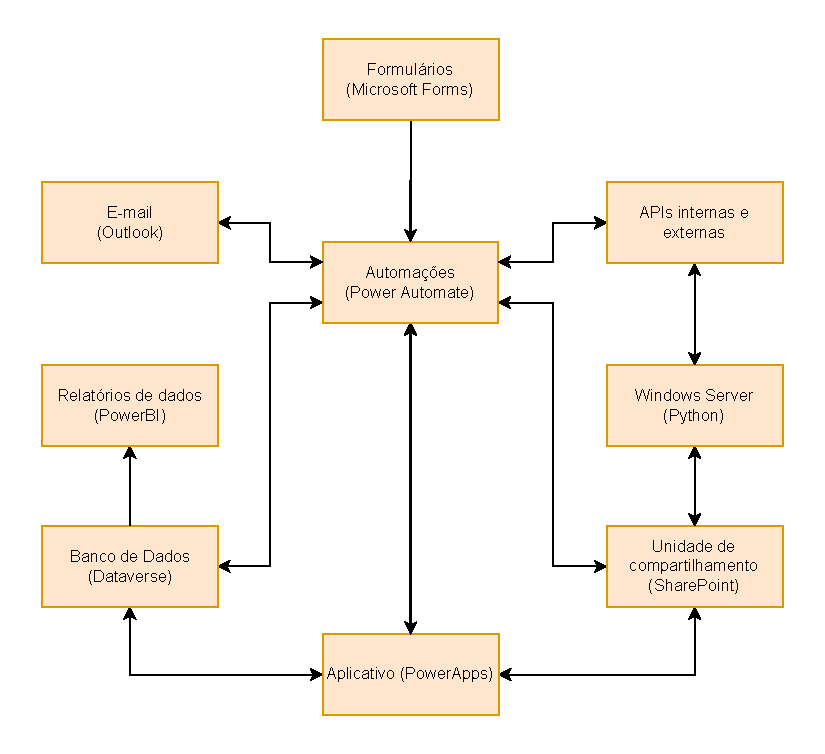
\includegraphics[width=1\textwidth]{./figuras/arquiteturaFisica.pdf}
		\caption{Padrão de arquitetura física dos sistemas desenvolvidos.}
		\label{fig:metodologia:arquiteturaFisica}
	\end{figure}

	Já na figura \ref{fig:metodologia:arquiteturaFuncional} temos o padrão de arquitetura funcional para os sistemas desenvolvidos, e mais uma vez, contém todas as possibilidades
	de funções disponíveis e que podem ser implementadas no sistema de interesse.
	\begin{figure}[h]
		\centering
		% \includegraphics[width=1\textwidth]{./figuras/scattering.eps}
		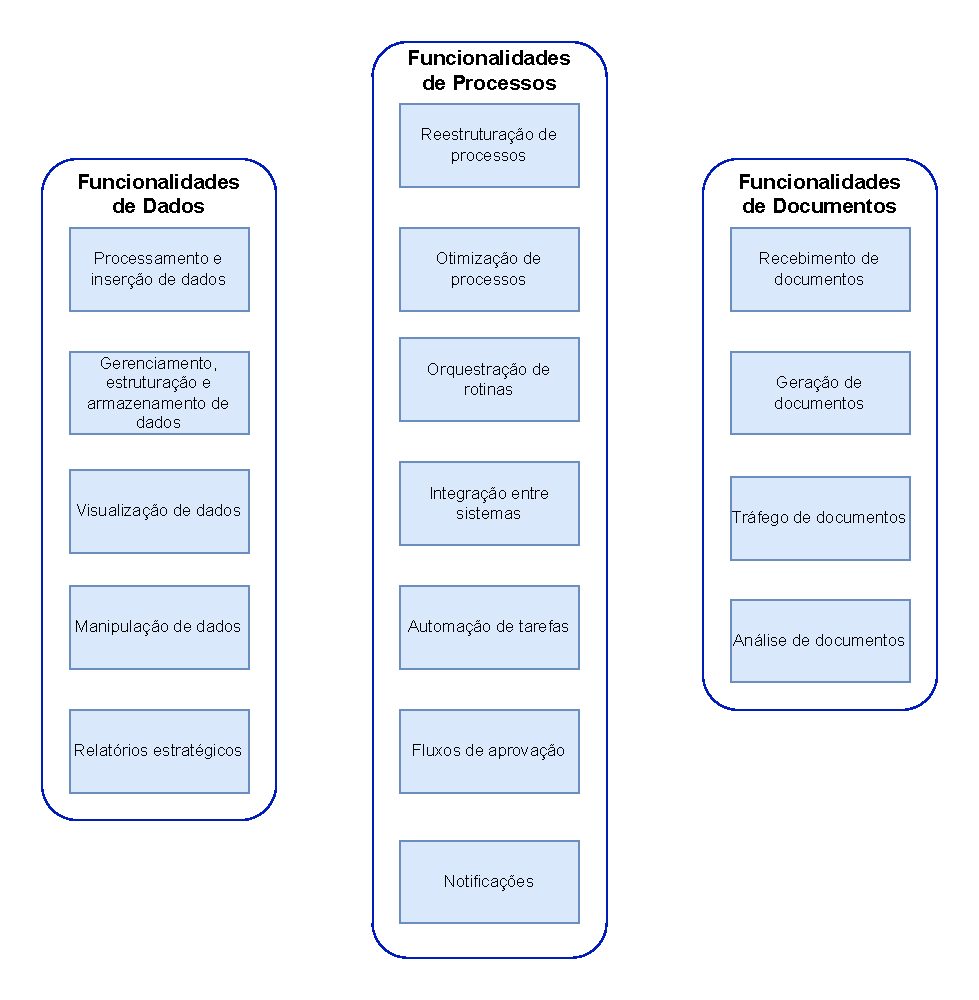
\includegraphics[width=1\textwidth]{./figuras/arquiteturaFuncional.pdf}
		\caption{Padrão de arquitetura funcional dos sistemas desenvolvidos.}
		\label{fig:metodologia:arquiteturaFuncional}
	\end{figure}

    % Resultados
    %% ------------------------------------------------------------------------------
% Resultados
% ------------------------------------------------------------------------------

\chapter{Resultados}\label{chap:resultados}

	O estudo e avaliação do processo de prestação do serviço nos moldes da Engenharia de Sistemas trouxe a clareza necessária para a proposição de sugestões de modificações no
	processo e a inclusão de ferramentas que auxiliam no gerenciamento dos sistemas desenvolvidos. 
	
	Seguindo os procedimentos para coleta de resultados, e aplicando as modificações no processo, foram gerados dados para avaliar o impacto do trabalho realizado, e comparar com medições
	previamente estabelecidas. 

	\section{Resultados para a criação de novas histórias de usuário}

	Ao serem confeccionadas as arquiteturas funcional e física para as novas soluções foram obtidos artefatos de grande importância para as
	fases de \textbf{Desenvolvimento Avançado} e \textbf{Projeto de Engenharia}. No caso da arquitetura física, foi de grande valia para a criação das
	histórias de usuário e tarefas a serem executadas. Nas Figuras \ref{fig:metodologia:solucaoXArqFis} e \ref{fig:metodologia:solucaoYArqFis} vemos as arquiteturas físicas para dois sistemas desenvolvidos seguindo
	a nova metodologia, as caixas de e-mail foram censuradas para preservar o sigilo.

	\begin{figure}[!h]
		\centering
		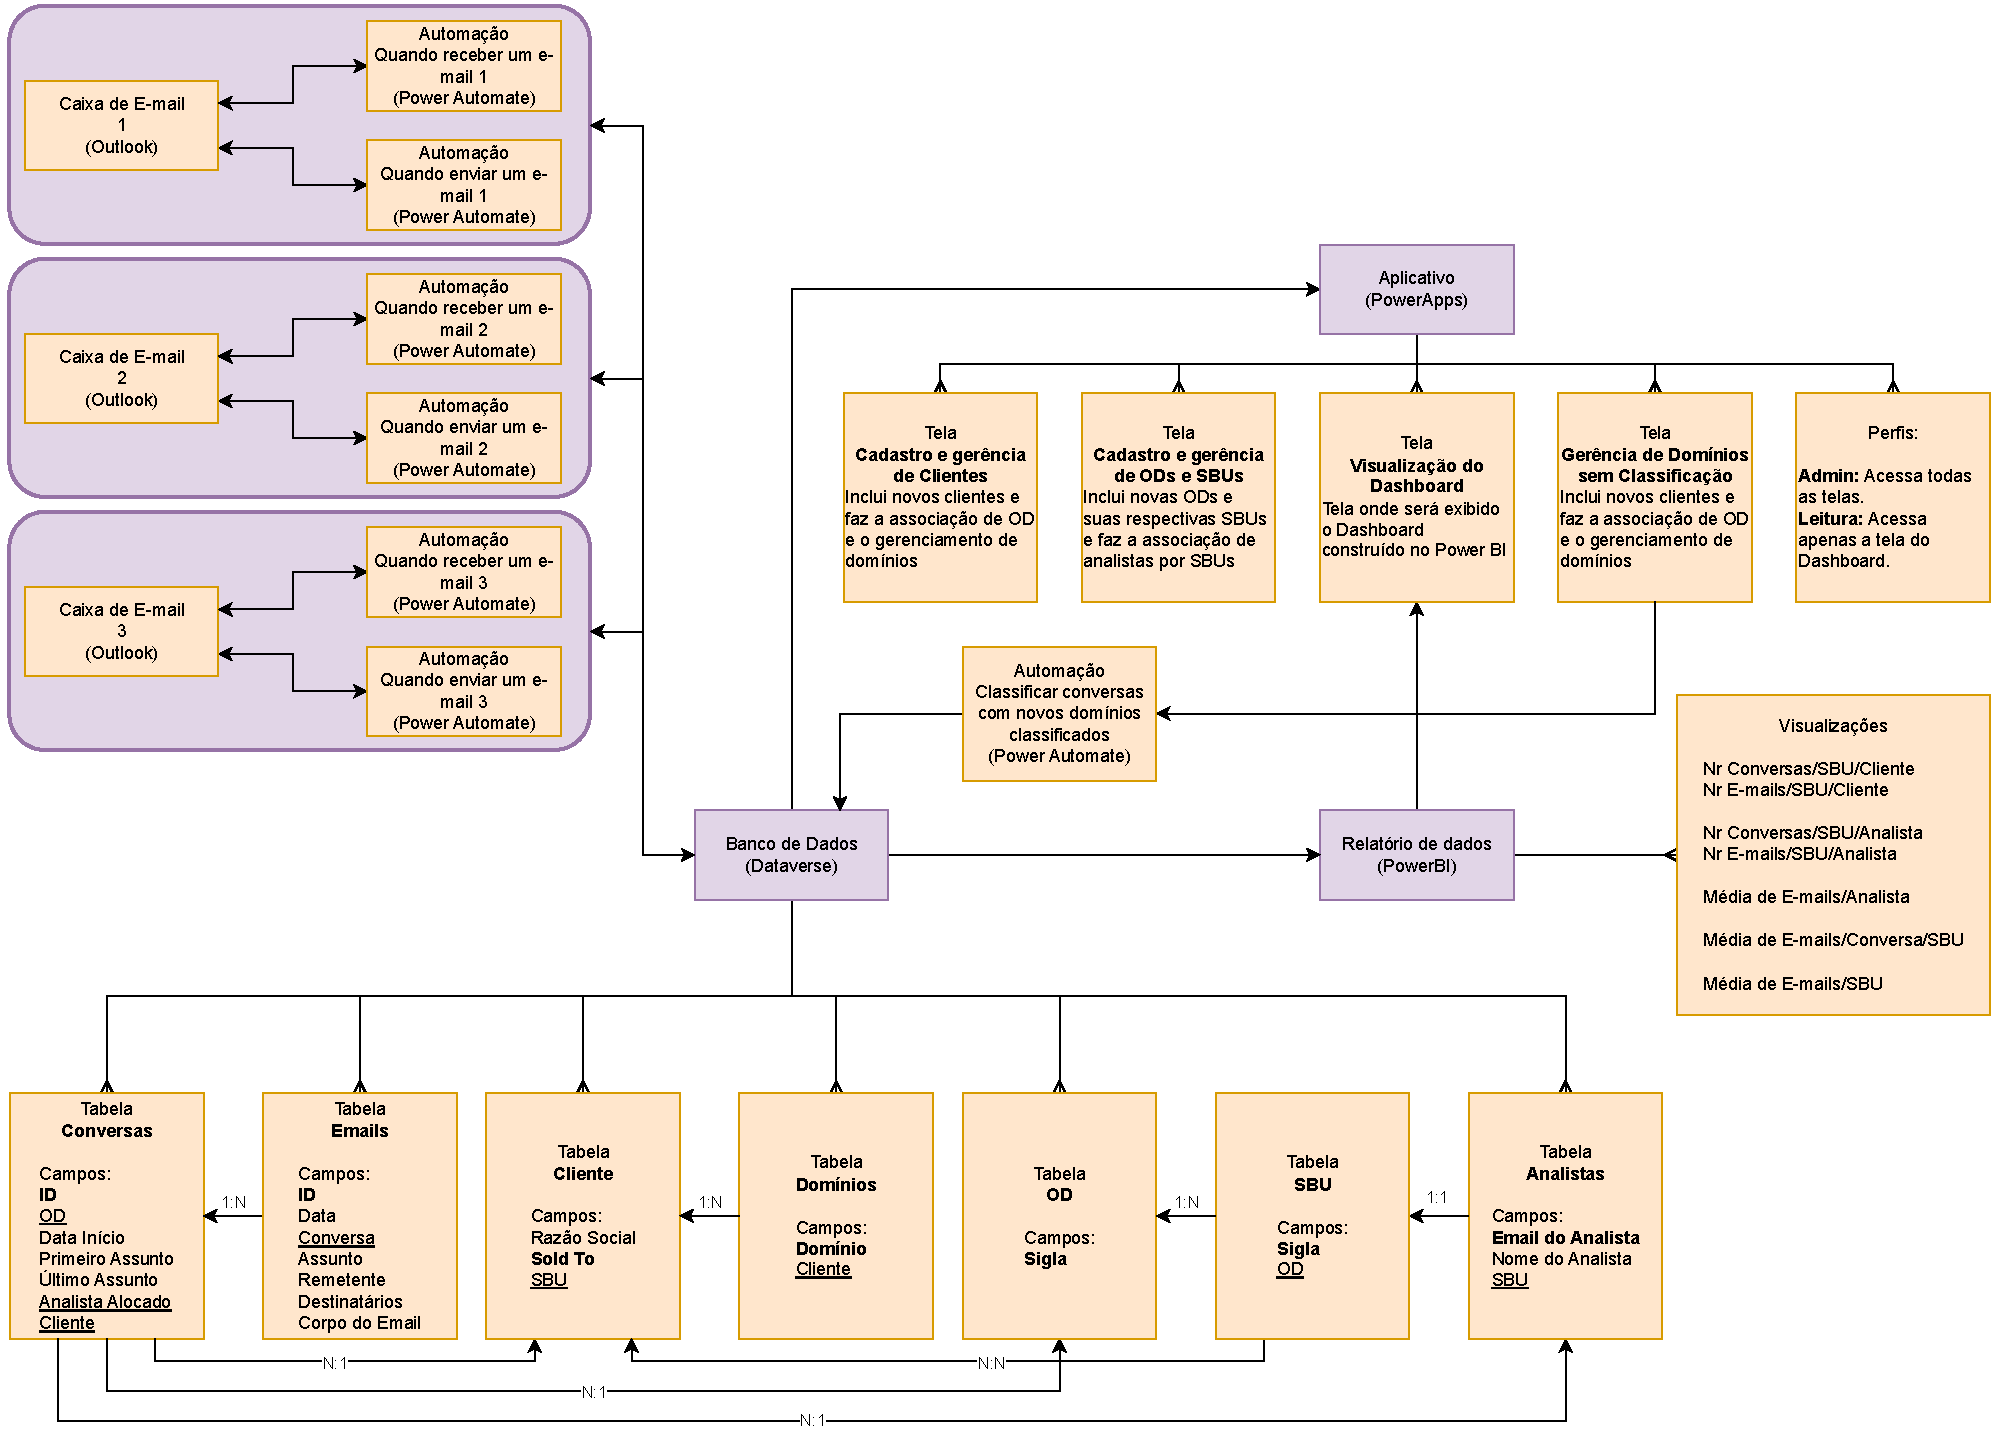
\includegraphics[width=1\textwidth]{./figuras/solucaoXArqFis.pdf}
		\caption{Arquitetura física da Solução X}
		\label{fig:metodologia:solucaoXArqFis}
	\end{figure}
	
	\begin{figure}[!h]
		\centering
		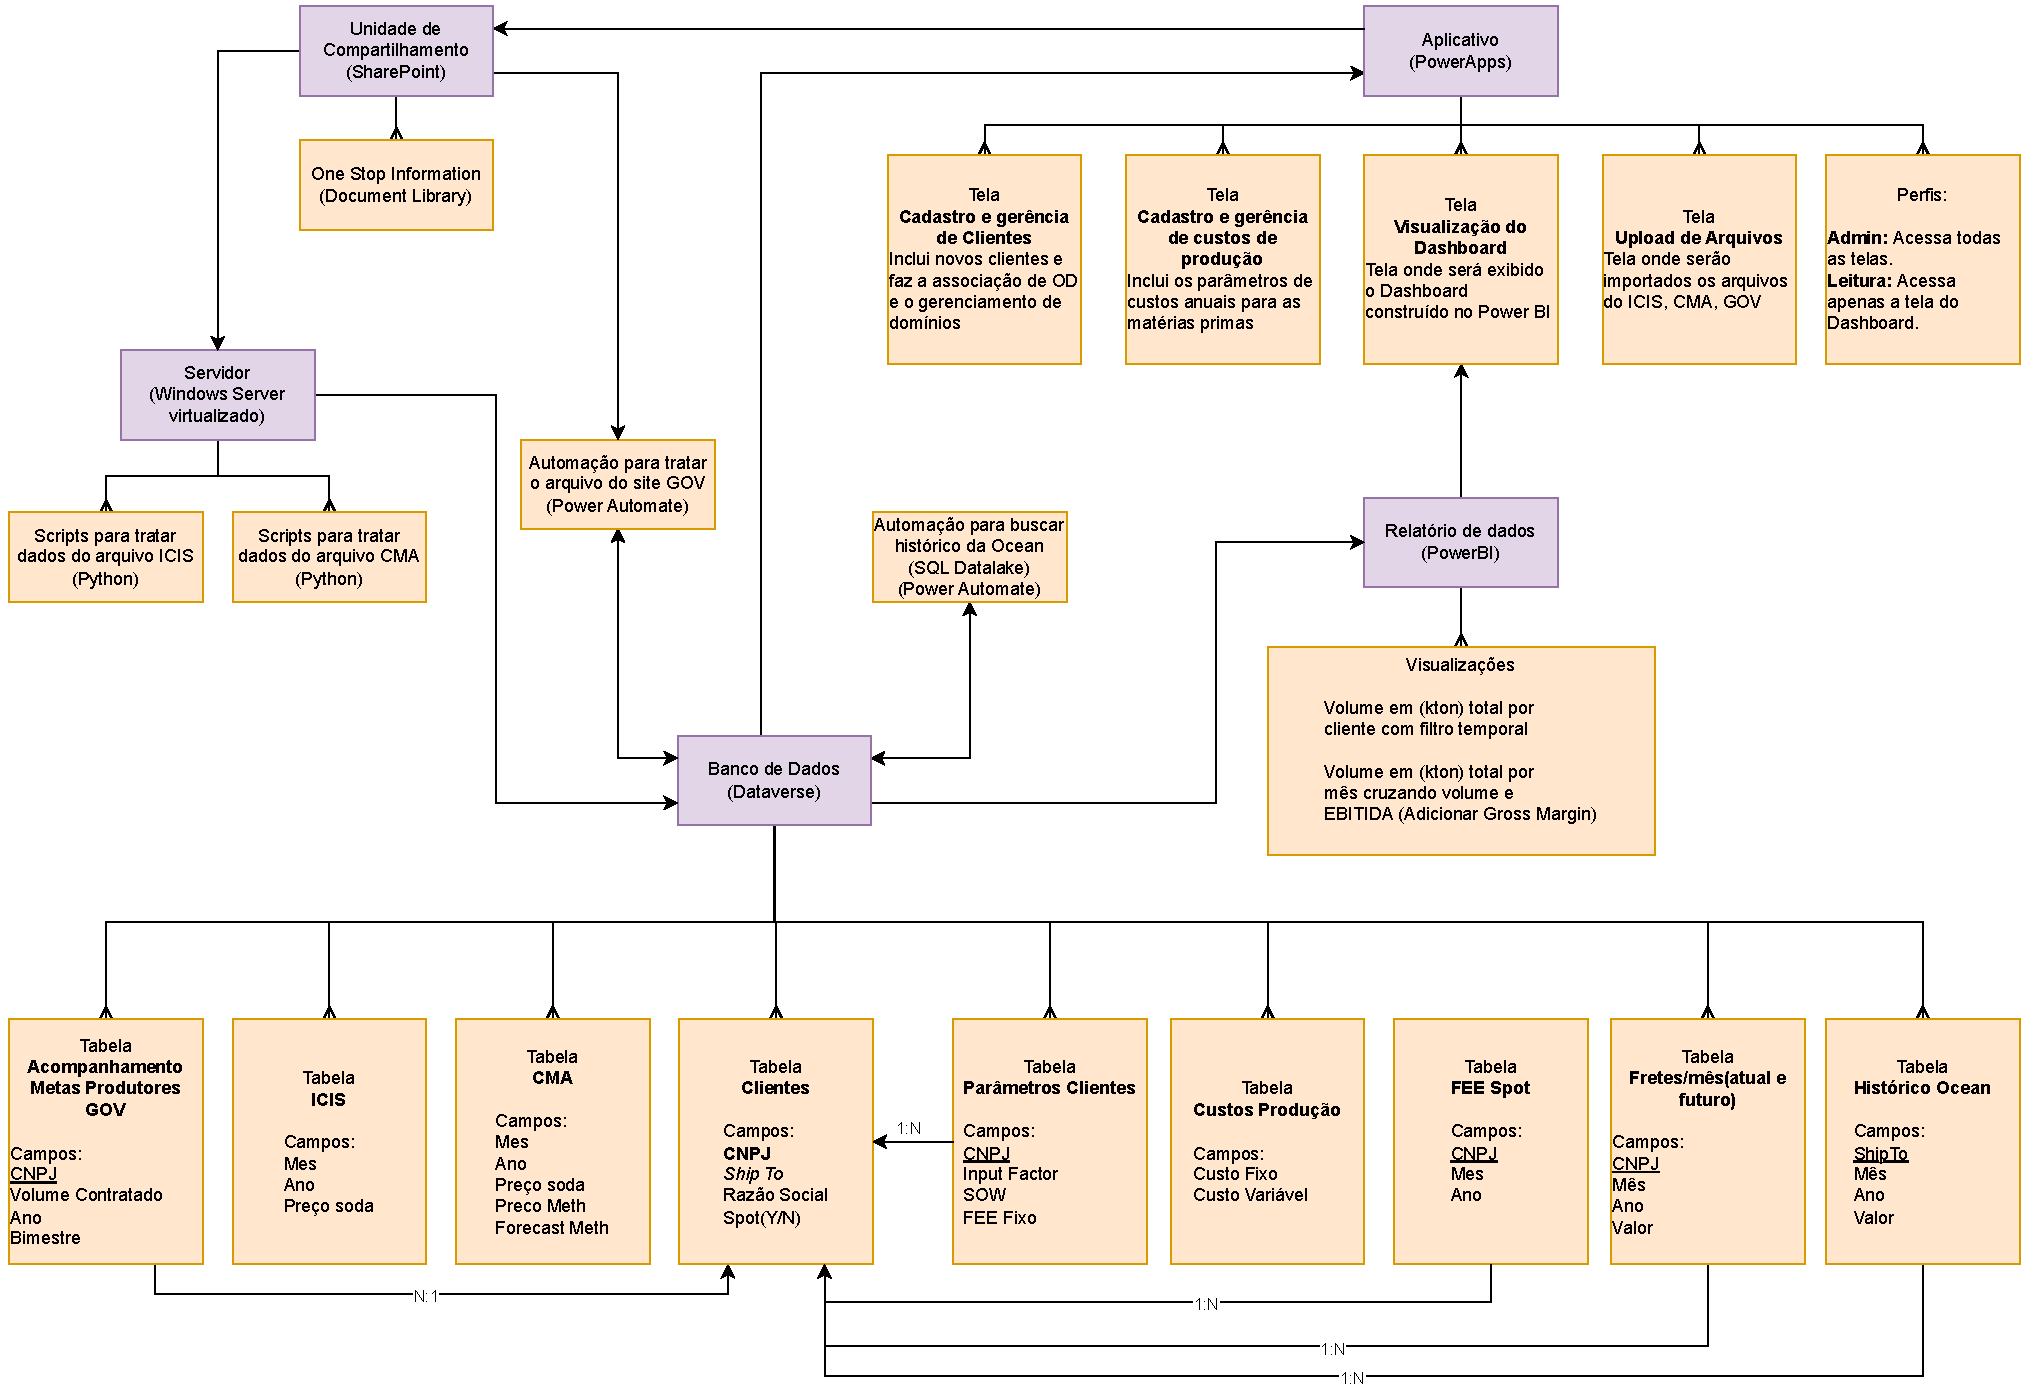
\includegraphics[width=1\textwidth]{./figuras/oneStopArqFis.pdf}
		\caption{Arquitetura física da Solução Y}
		\label{fig:metodologia:solucaoYArqFis}
	\end{figure}

	Baseado nessas arquiteturas, foram criadas as tarefas de cada história de usuário e definido os pontos de esforço. Na Tabela \ref{tab:esforco_solucoes_resultado} foi incluído
	também o aplicativo construído para a rastreabilidade como a Solução Z.

	\begin{longtable}{cccccc}
		\label{tab:esforco_solucoes_resultado} \\
		\toprule
		\textbf{ID} & \textbf{Solução} & \textbf{Categoria} & \textbf{Tarefas} & \textbf{Pontos} & \textbf{Pontos por Tarefa} \\
		\midrule
		\endfirsthead

		\toprule
		\textbf{ID} & \textbf{Solução} & \textbf{Categoria} & \textbf{Tarefas} & \textbf{Pontos} & \textbf{Pontos por Tarefa} \\
		\midrule
		\endhead

		\midrule
		\multicolumn{6}{r}{\textit{continua na próxima página}} \\
		\midrule
		\endfoot

		\bottomrule
		\caption{Distribuição de esforço por solução e categoria}
		\endlastfoot

		178690 & X & Automação & 10 & 10 & 1.00 \\
		178750 & X & Automação & 10 & 10 & 1.00 \\
		178766 & X & Automação & 10 & 10 & 1.00 \\
		178830 & X & Automação & 3 & 5 & 1.67 \\
		179009 & Y & Automação & 2 & 3 & 1.50 \\
		179010 & Y & Automação & 2 & 5 & 2.50 \\
		179011 & Y & Automação & 2 & 2 & 1.00 \\
		178707 & X & Banco de dados & 7 & 13 & 1.86 \\
		179005 & Y & Banco de dados & 12 & 16 & 1.33 \\
		179020 & Z & Banco de dados & 4 & 6 & 1.50 \\
		178825 & X & Relatório de dados & 5 & 15 & 3.00 \\
		179006 & Y & Relatório de dados & 8 & 18 & 2.25 \\
		179007 & Y & Script & 3 & 8 & 2.67 \\
		179008 & Y & Script & 3 & 8 & 2.67 \\
		178784 & X & Tela & 9 & 16 & 1.78 \\
		178795 & X & Tela & 9 & 19 & 2.11 \\
		178806 & X & Tela & 5 & 7 & 1.40 \\
		178814 & X & Tela & 9 & 17 & 1.89 \\
		179001 & Y & Tela & 4 & 12 & 3.00 \\
		179002 & Y & Tela & 5 & 12 & 2.40 \\
		179003 & Y & Tela & 6 & 13 & 2.17 \\
		179004 & Y & Tela & 4 & 5 & 1.25 \\
		179021 & Z & Tela & 3 & 5 & 1.67 \\
		179022 & Z & Tela & 2 & 4 & 2.00 \\
		179023 & Z & Tela & 3 & 5 & 1.67 \\
	\end{longtable}


	\begin{table}[!htb]
		\centering
		\begin{tabular}{ccc}
			\toprule
			\textbf{Categoria} & \textbf{Média de Pontos/Tarefas} & \textbf{Desvio Padrão de Pontos/Tarefas} \\
			\midrule
			Automação          & 1.38                             & 0.57                                 \\
			Banco de dados     & 1.56                             & 0.07                                 \\
			Relatório de dados & 2.63                             & 0.28                                 \\
			Script             & 2.67                             & 0.00                                 \\
			Tela               & 2.00                             & 0.51                                 \\
			\bottomrule
		\end{tabular}
		\caption{Média e variância dos pontos de esforço por categoria após aplicação das mudanças sugeridas}
		\label{tab:media_variancia_resultado}
	\end{table}

	É notável que houve uma queda nas médias de pontos por tarefas em todas as categorias de desenvolvimento ao se comparar com as mesmas estatísticas dos dados históricos mostrados na Tabela
	\ref{tab:media_desvio_historico}. Nota-se também uma queda no desvio padrão de cada categoria, no caso da categoria Script, observa-se um valor nulo, pois as duas atividades de desenvolvimento nessa categoria
	possuíam os mesmos números de tarefas e esforço, e como são, ainda por cima, da mesma solução, não trazem consigo uma representatividade suficiente para serem levados em consideração como um ganho.

	Para as outras categorias, no entanto, esses valores representam uma distribuição mais uniforme de esforço por tarefa e um nível de detalhamento maior. Esse resultado anda paralelo a 
	um melhor entendimento do serviço a ser executado.

	Nas reuniões para validação da solução com as áreas clientes, ou simplesmente a validação de conceito, a arquitetura física foi de grande ajuda para o engajamento do pessoal. As partes interessadas
	foram capazes de opinar e sugerir alterações, visto que o nível de detalhamento apresentado não chegou a um nível inascessível. Além disso, ela funciona como um documento comprobatório do escopo do projeto, evitando  de forma {\color{red} ???}, a
	inclusão de novas fucionalidades fora do escopo, que não estão acomodades no sistema projetado e definido.


	Além dos dados numéricos apresentados, vale ressaltar que com a documentação das arquiteturas funcionais e físicas, foi viabilizado a utilização do auxílio
	do agente de IA autônomo (\textit{Microsoft Copilot}) para a criação das histórias de usuários. Ao serem enviados os documentos das arquiteturas com um \text{prompt} contextualizando sobre a solução e
	a estrutura e ferramentas de trabalho da equipe, o agente foi capaz de gerar as histórias de usuário e suas tarefas com bastante exatidão, e poucas alterações durante a
	revisão das mesmas, basicamente sendo necessária apenas a exclusão de tarefas desnecessárias, a unificação de tarefas pequenas e muito relacionadas, ou a inclusão de poucas tarefas não consideradas.

	\begin{table}[!htb]
		\centering
		\begin{tabular}{cccc}
			\toprule
			\textbf{Solucão} & \textbf{Tarefas Sugeridas} & \textbf{Tarefas Utilizadas} & \textbf{Diferença percentual} \\
			\midrule
			X & 92  & 77 & -16.3\% \\
			Y & 44  & 51 & 13.7\% \\
			Z & 12  & 12 & 0\% \\
			\bottomrule
		\end{tabular}
		\caption{Quantidade de tarefas geradas pelo agente de IA, a quantidade realmente utilizada e a Diferença percentual}
		\label{tab:tarefas_copilot}
	\end{table}
	
	É visto um bom aproveitamento da tarefas sugeridas, e nota-se que para soluções menos complexas o agente autônomo foi mais assertivo nas tarefas a serem executadas. Esse tipo de
	ação e colaboração com IA trás uma economia de tempo e recurso muito significativa, onde antes o desenvolvedor deveria criar toda a estrutura, e agora apenas revisa e faz pequenas alterações,
	sobrando então mais tempo para atividades de desenvolvimento de fato.

	\section{Resultados para Rastreabilidade}

	A proposta de criar uma aplicação para garantir a rastreabilidade do sistema traz valor em fases mais avançadas do ciclo de vida, em especial as fases de utilização e suporte. Caso surja
	alguma melhoria ou manutenção nessas etapas, o custo envolvido nessas mudanças é maior que se fossem feitas durante a fase de produção, no caso o custo é o equivalente ao esforço empenhado nessas
	mudanças. Então, saber exatamente o impacto dessas alterações no sistema se torna crucial para uma ação consciente e responsável.

	O aplicativo construído pode ser observado nas Figuras \ref{fig:resultados:solucoes} a \ref{fig:resultados:dependenciaCruzada}.

	\begin{figure}[!h]
		\centering
		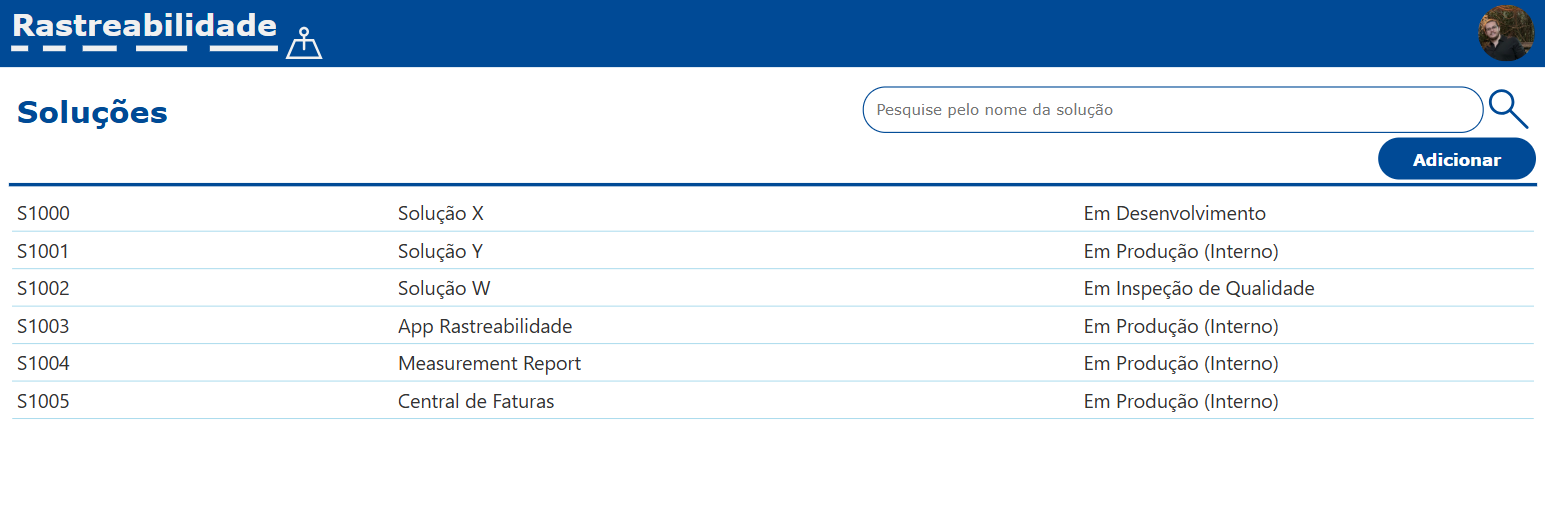
\includegraphics[width=1\textwidth]{./figuras/solucoes.png}
		\caption{Tela de visualização das soluções.}
		\label{fig:resultados:solucoes}
	\end{figure}

	\begin{figure}[!h]
		\centering
		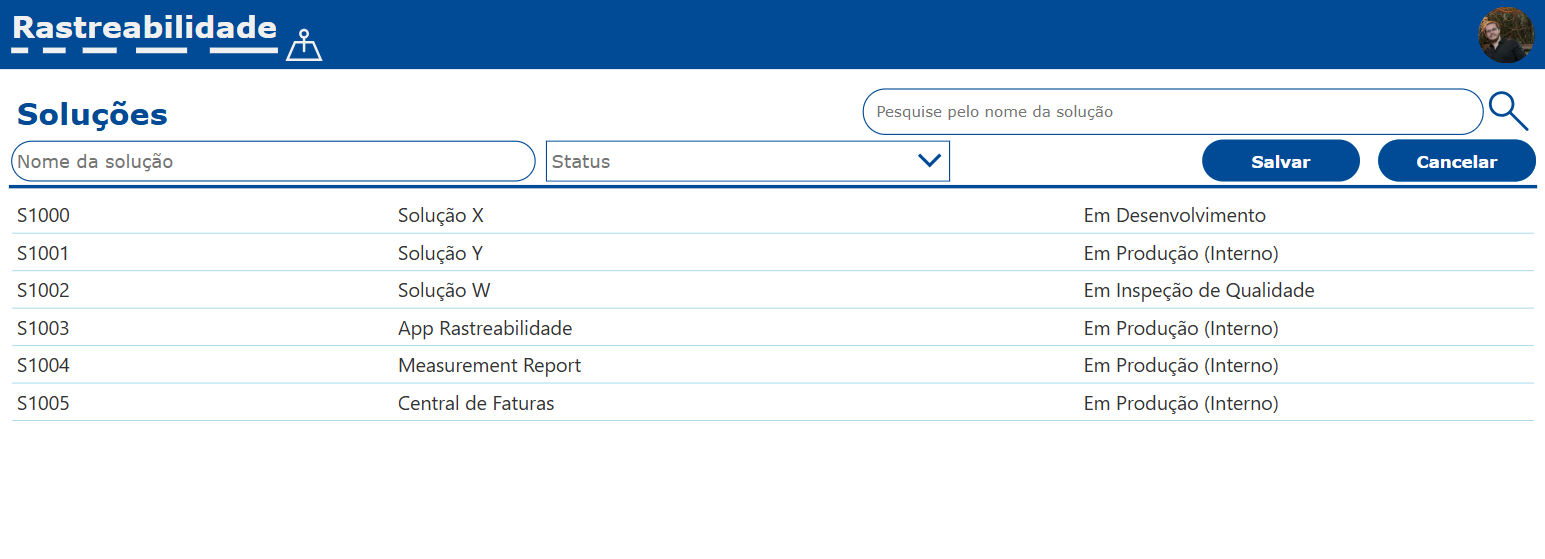
\includegraphics[width=1\textwidth]{./figuras/solucoesAdicionar.png}
		\caption{Tela de visualização das soluções com a expansão dos campos para adicionar nova solução.}
		\label{fig:resultados:solucoesAdicionar}
	\end{figure}

	\begin{figure}[!h]
		\centering
		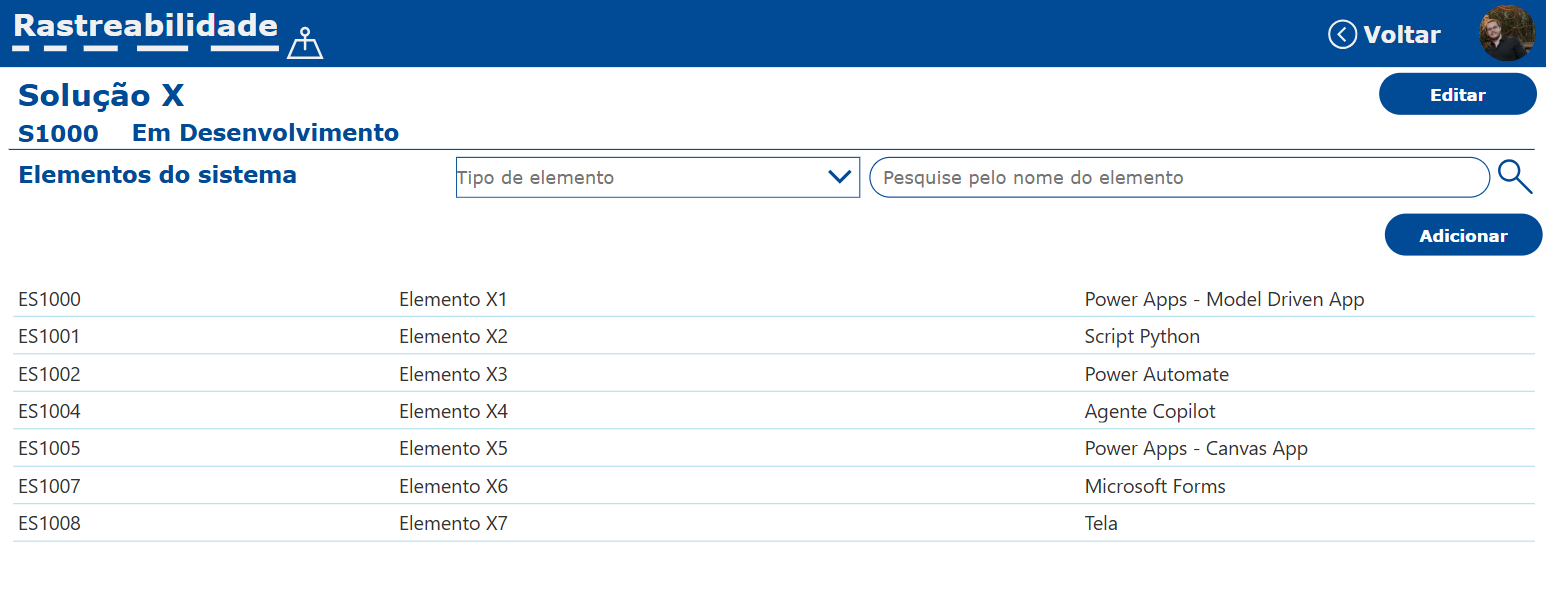
\includegraphics[width=1\textwidth]{./figuras/solucaoElementos.png}
		\caption{Tela de visualização dos elementos.}
		\label{fig:resultados:solucaoElementos}
	\end{figure}

	\begin{figure}[!h]
		\centering
		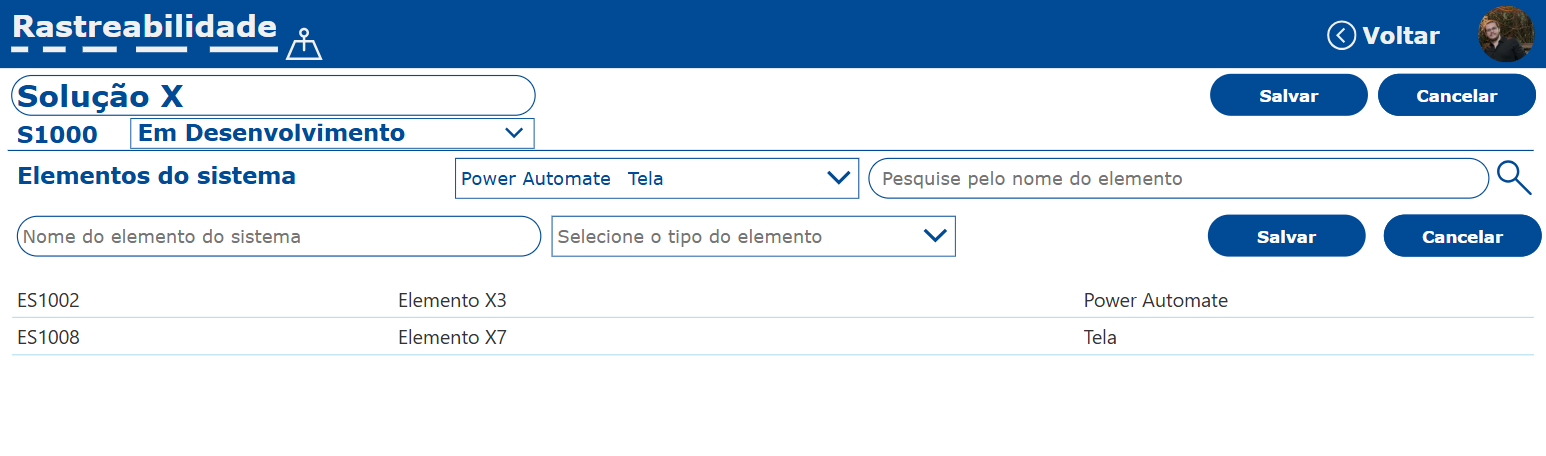
\includegraphics[width=1\textwidth]{./figuras/solucaoElementosAdd.png}
		\caption{Tela de visualização dos elementos com a expansão dos campos para adicionar novo elemento e editar dados da soluçao atual.}
		\label{fig:resultados:solucaoElementosAdd}
	\end{figure}

	\begin{figure}[!h]
		\centering
		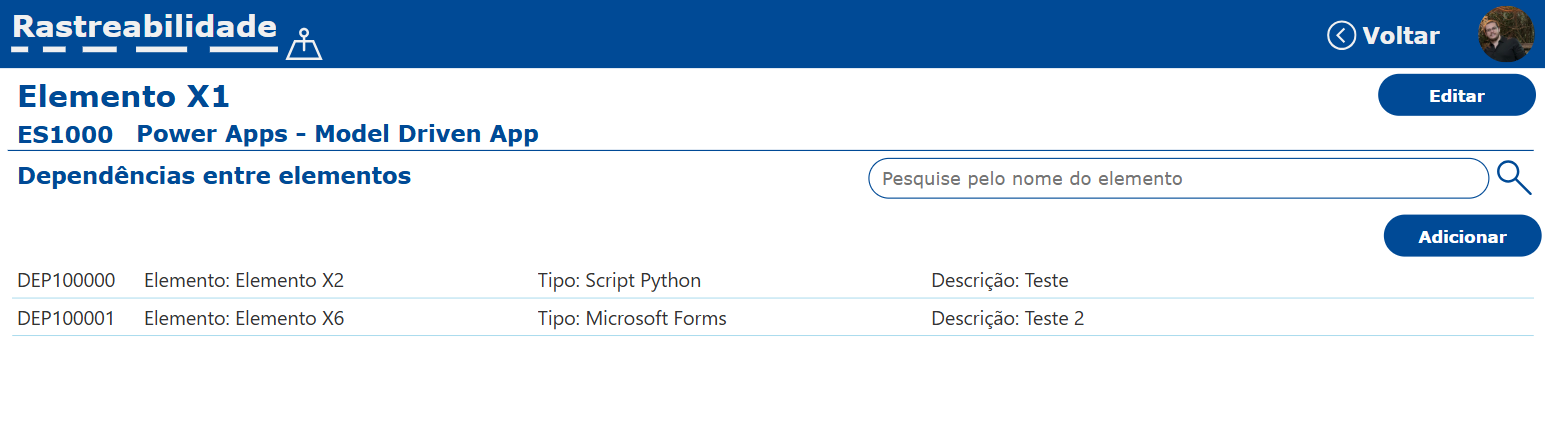
\includegraphics[width=1\textwidth]{./figuras/elementoDependencias.png}
		\caption{Tela de visualização das dependências.}
		\label{fig:resultados:elementoDependencias}
	\end{figure}

	\begin{figure}[!h]
		\centering
		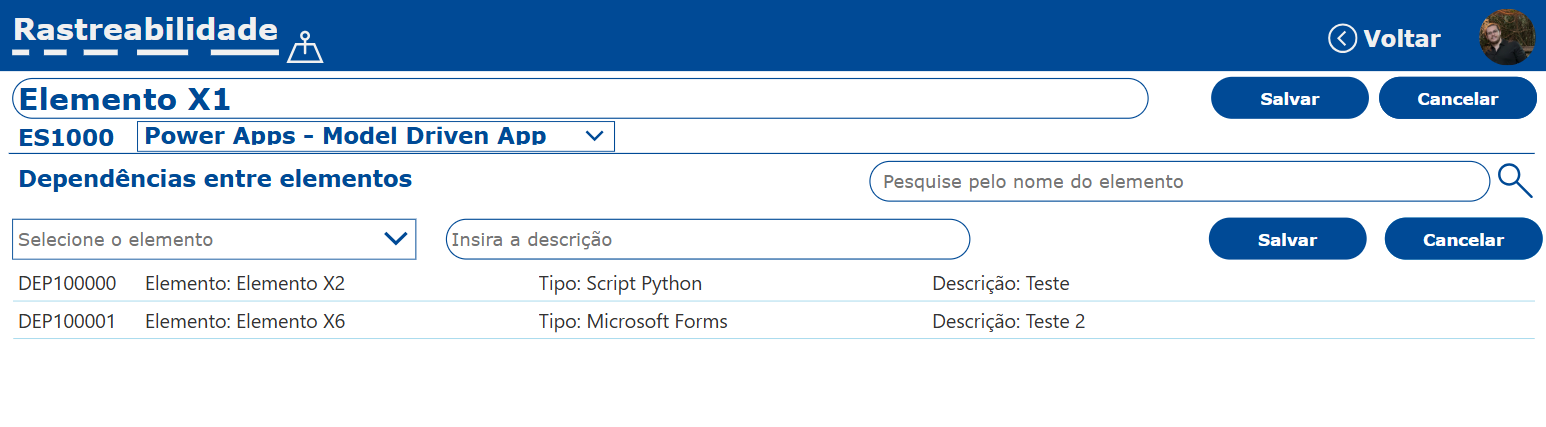
\includegraphics[width=1\textwidth]{./figuras/elementoDependenciasAdd.png}
		\caption{Tela de visualização das dependências com a expansão dos campos para adicionar nova dependência e editar o elemento atual}
		\label{fig:resultados:elementoDependenciasAdd}
	\end{figure}

	\begin{figure}[!h]
		\centering
		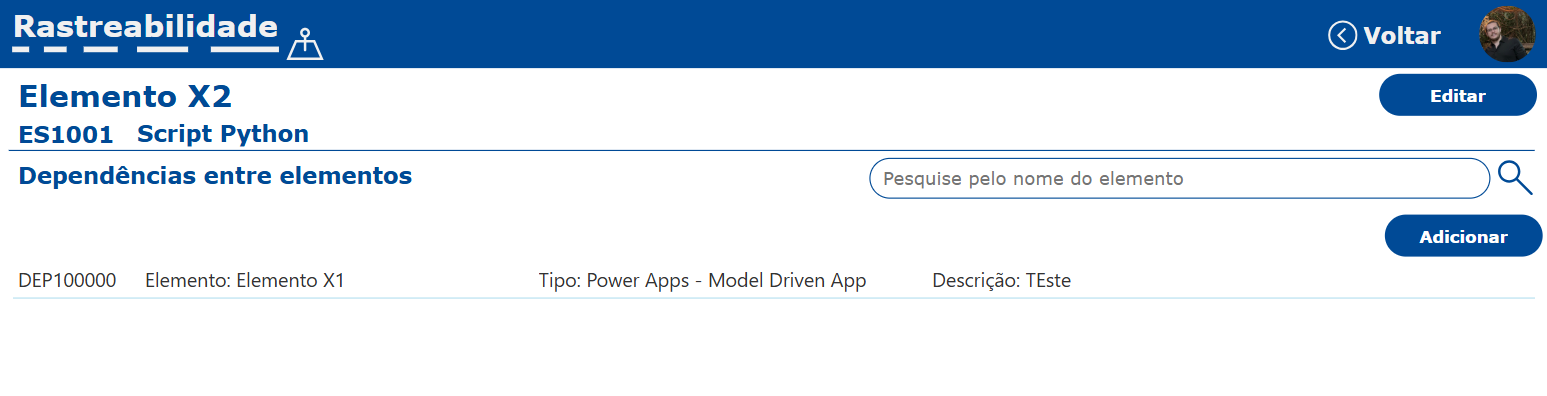
\includegraphics[width=1\textwidth]{./figuras/dependenciaCruzada.png}
		\caption{Tela de visualização evidenciando a dependência cruzada.}
		\label{fig:resultados:dependenciaCruzada}
	\end{figure}

	Como sugerido, foram propostos três cenários para avaliação de esforço de atuação:

	\begin{itemize}
		\item \textbf{Cenário 1:} O fluxo de automação que envia o resultado da análise das notas fiscais para o fornecedor e as notas aprovadas para {\color{red} pamaneto},
		foi deletado por engano e precisa ser feito novamente.
		\item \textbf{Cenário 2:} A caixa compartilhada de e-mail utilizada para as notificações do sistema precisa ser substituída por outra.
		\item \textbf{Cenário 3:} A inclusão de uma coluna com dado importante em uma tabela que deve ser exibida junto com as outras informações provenientes dessa tabela, seja no e-mail ou no próprio aplicativo.
	\end{itemize}

	As imagens \ref{fig:resultados:sendReviewedResponse}, \ref{fig:resultados:caixadeEmail} e \ref{fig:resultados:solicitacoesTabela} mostram as telas do aplicativo
	que foram mostradas para cada cenário antes da reavaliação pelo desenvolvedores.

	\begin{figure}[!h]
		\centering
		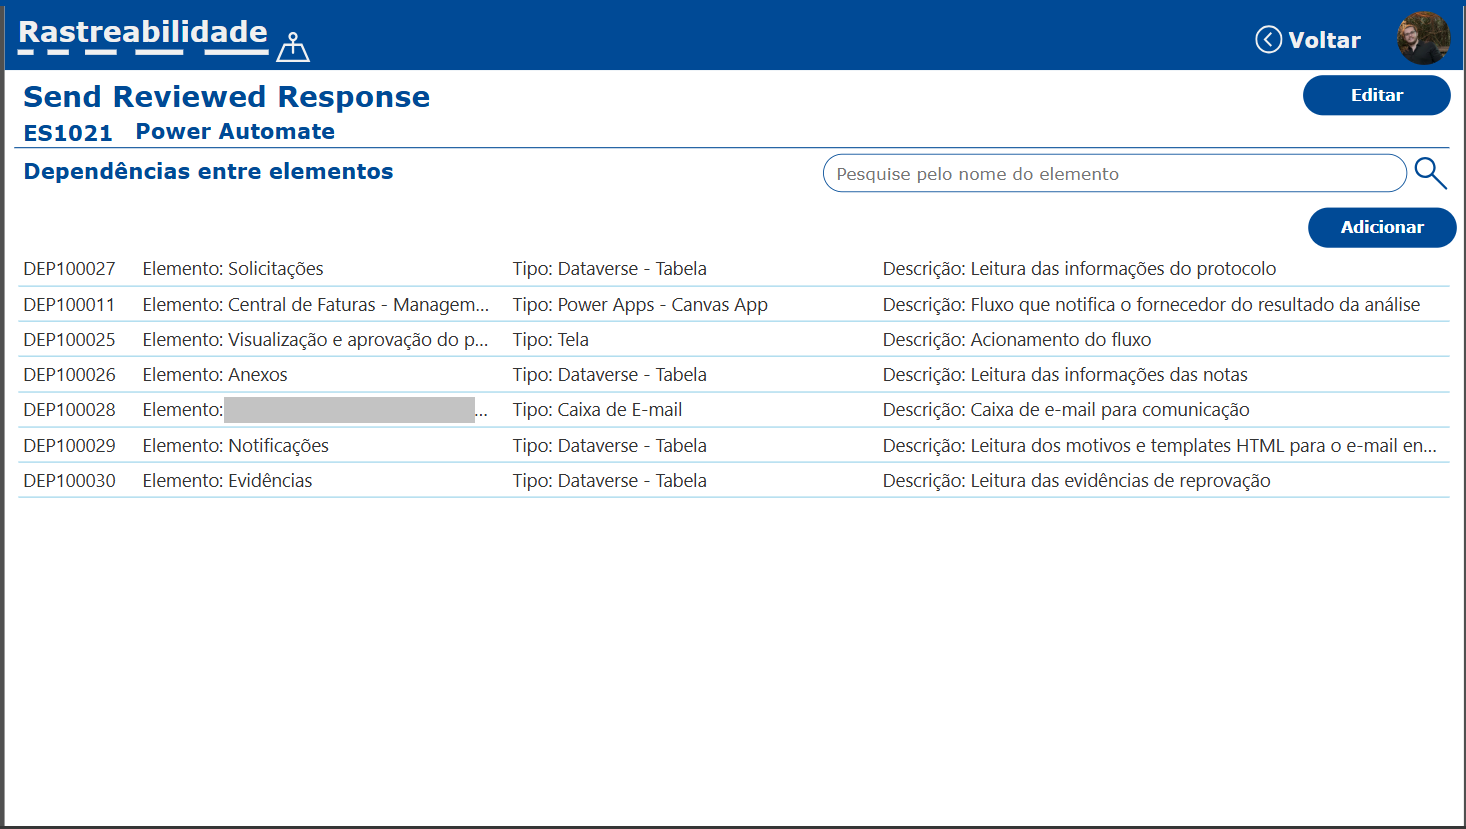
\includegraphics[width=1\textwidth]{./figuras/sendReviewedResponse.png}
		\caption{Dependências relacionadas ao Cenário 1}
		\label{fig:resultados:sendReviewedResponse}
	\end{figure}

	\begin{figure}[!h]
		\centering
		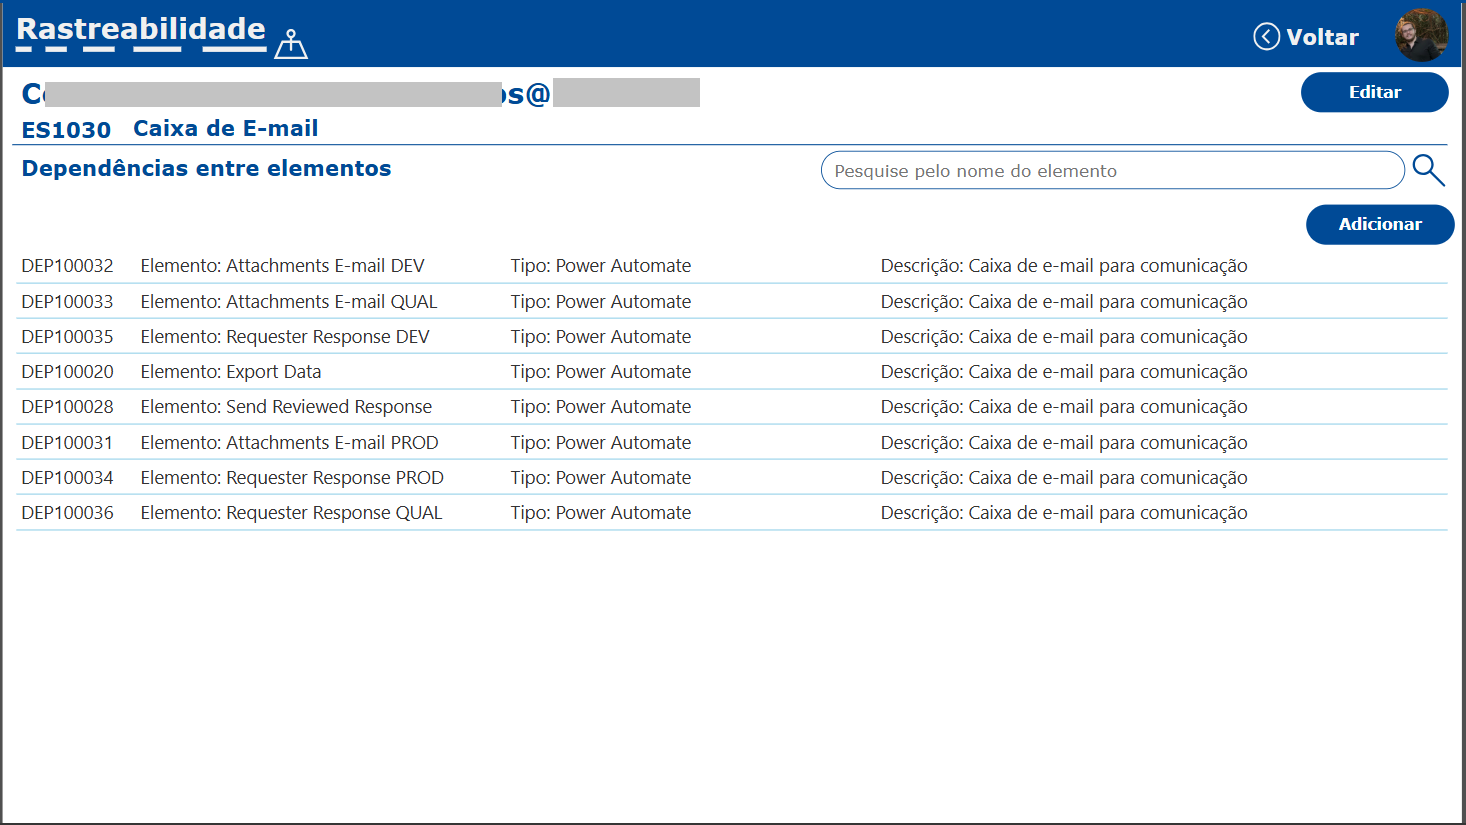
\includegraphics[width=1\textwidth]{./figuras/caixadeEmail.png}
		\caption{Dependências relacionadas ao Cenário 2}
		\label{fig:resultados:caixadeEmail}
	\end{figure}

	\begin{figure}[!h]
		\centering
		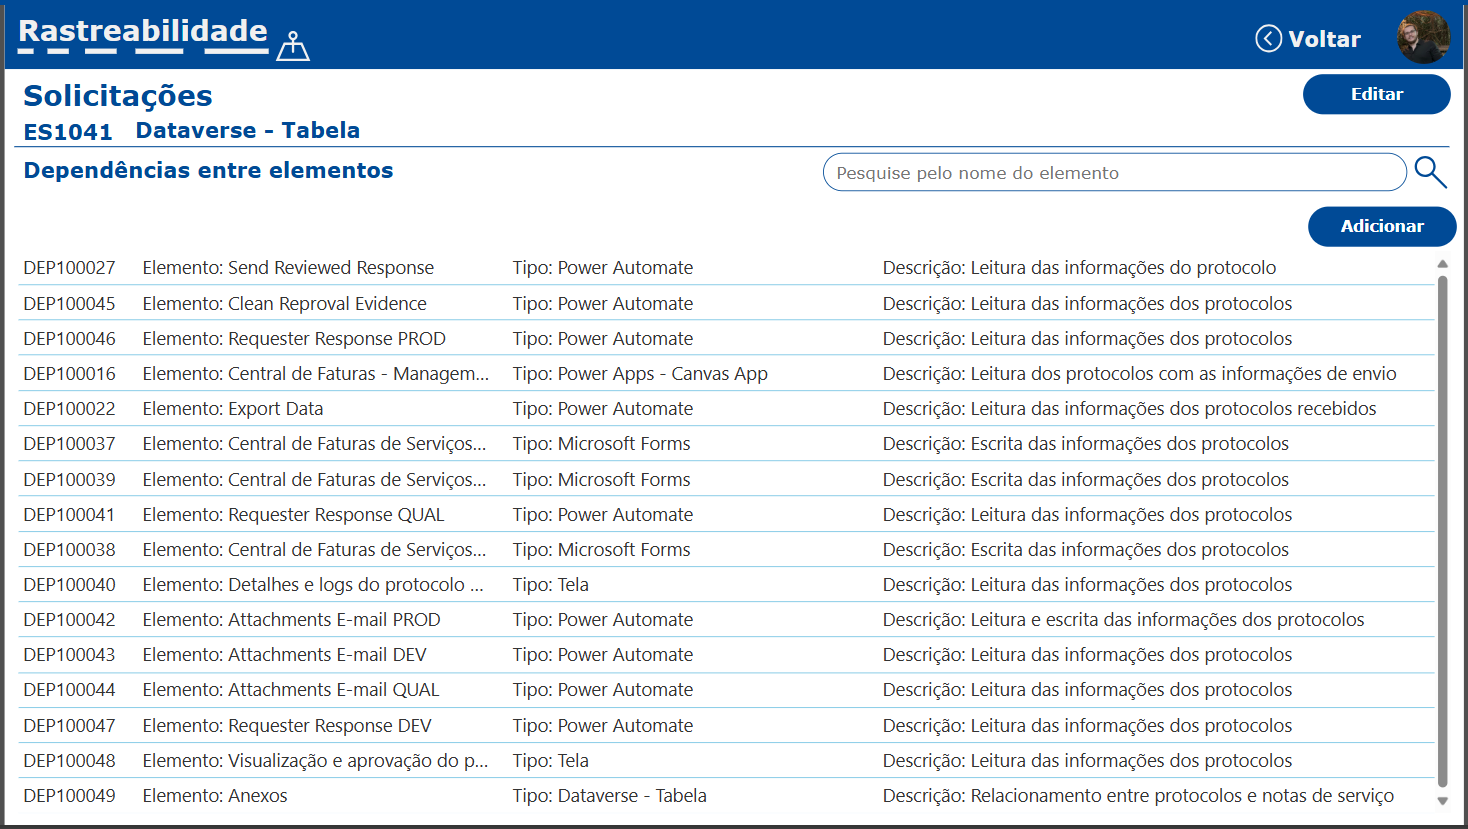
\includegraphics[width=1\textwidth]{./figuras/solicitacoesTabela.png}
		\caption{Dependências relacionadas ao Cenário 3}
		\label{fig:resultados:solicitacoesTabela}
	\end{figure}

	Na Tabela \ref{tab:cenarios_desenvolvimento} podem ser vistos os valores atribuídos a cada cenário antes e depois da apresentação do aplicativo.

	\begin{table}[!htb]
		\centering
		\begin{tabular}{c cc cc cc}
			\toprule
			\textbf{Desenvolvedor} & \multicolumn{2}{c}{\textbf{Cenário 1}} & \multicolumn{2}{c}{\textbf{Cenário 2}} & \multicolumn{2}{c}{\textbf{Cenário 3}} \\
			& Antes & Depois & Antes & Depois & Antes & Depois \\
			\midrule
			1 & 5 & 5 & 1 & 2 & 3 & 5 \\
			2 & 8 & 8 & 1 & 3 & 3 & 8 \\
			3 & 5 & 8 & 1 & 1 & 3 & 5 \\
			\midrule
			Média & 6 & 7 & 1 & 2 & 3 & 6 \\
			Desvio Padrão & 1.73 & 1.73 & 0.00 & 1.00 & 0.00 & 1.73 \\
			\bottomrule
		\end{tabular}
		\caption{Comparativo do esforço alocado em três cenários, antes e depois do uso do aplicativo}
		\label{tab:cenarios_desenvolvimento}
	\end{table}

	Apesar de indicado o desvio padrão para as medidas, não se extrai muita informação dessa comparação visto que foram poucas amostragens de esforço e o valor variou pouco,
	caso um grande número de desenvovedores forem envolvidos faria mais sentido essa métrica. No entanto, ao olharmos para a média das avalições, ou mesmo individualmente por
	desenvolvedor, após a apresentação do aplicativo, na reavaliação, os valores sobem em quase todos os casos individuais e em todos os casos de média.

	Isso mostra um aumento na percepção de esforço a ser empenhado quando se tem clareza das dependências envolvidas na ação que se pretende realizar.

	
	\begin{itemize}		
		\item {\color{red} Sumário dos Resultados: Conclua o capítulo com um sumário dos principais resultados.}
	\end{itemize}

    % Conclusão
    %% ------------------------------------------------------------------------------
% Conclusão
% ------------------------------------------------------------------------------

\chapter{Conclusão}\label{chap:conclusao}
	
	Os conceitos e boas práticas da Engenharia de Sistemas são versáteis e podem ser aplicados em diversos tipos de ambientes e organizações. O trabalho realizado mostra
	que mesmo em cenários bem específicos e fora dos padrões tradicionais, há ganhos na análise do ciclo de vida sob a ótica da ES. Essa análise permite uma tomada de decisao mais embasada e acertiva
	nas mudanças sugeridas, que por sua vez, mostram-se efetivas em reduzir os problemas iniciais identificados, na definicão e validação do conceito e na rastreabilidade dos componentes do sistema.

	{\color{red}Contextualização}
	
	A autonomia concedida para a aplicação das modificações do ciclo de vida foram de extrema importância para o trabalho, sem isso não seria possível a análise de dados reais da equipe. Ser o membro da equipe
	técnica com mais senioridade do time e o número reduzido de pessoas facilitou a implantação das mudanças e a aceitação do restante da equipe, que poderia ser um desafio considerável
	em times maiores ou com pessoas mais experientes já ambientadas com o processo antigo, mesmo este sendo problemático. Um ponto a se destacar é que o novo ciclo de vida foi aplicado em apenas dois sistemas reais
	para área clientes e ao próprio aplicativo desenvolvido nesse trabalho, e não chegou a ser concluído ainda para nenhum dos sistemas. Logo a representatividade dos dados ainda não tem um nível grande de maturidade
	em uma visão macro do serviço de criação de sistemas.

	Os resultados encontrados reforçam a importância de um ciclo de vida bem estruturado e ademais, a importância das fases de Definicão do Conceito e Desenvolvimento Avançado, principalmente em projetos de escopo fechado.
	No caso dos sistemas desenvolvidos que possuem um tempo de projeto atipicamente curto, essas duas fases tem um impacto maior ainda, pois qualquer erro na estimativa de esforço significa um alto percentual de atraso na entrega final.
	Uma melhor distribuição de esforço por tarefa como foi encontrado, ajuda na redução desse erro pois aumenta a granularidade das ações que devem ser executadas. Isso contribui ainda com uma maior visibilidade ao gerente de projetos, para realizar um trabalho de gerenciamento de riscos de projeto mais acertivo.
	Um outro ganho operacional foi a possibilidades da aplicação de IA na rotina de trabalho, que vai de encontro com os movimentos do mercado de buscar a redução do tempo empenhado em tarefas que podem ser feitas por esse tipo de ferramenta.

	Uma ferramenta para manutenção da rastreabilidade do sistema, como o aplicativo desenvolvido, juntamente com o resultado do aumento da estimativa de esforço após a utilização do mesmo, implica em uma redução de uma percepção de esforço muito otimista.
	Isso minimiza uma carga excessiva de trabalho ao alocar essas tarefas, inicialmente simples, para serem executas em conjunto com outras, e depois ela se tornar mais trabalhosa que o esperado.
	Essa visão da rastreabilidade melhora também o gerenciamento de riscos técnicos ao se planejar uma manuentenção ou na inclusão de uma melhoria em um sistema já existente.

	Para trabalhos futuros podem ser observados o efeito no prazo efetivo para a conclusão dos projetos de sistemas com essas mudanças no ciclo de vida. É um ponto de avanço incluir além dos elementos do sistema no aplicativo de rastreabilidade, as funcionalidades relacionadas acima deles, para tornar mais completa a hierarquia.
	Uma análise com mais dados seria de bom proveito também, principalmente na comparação de esforço na parte da rastreabilidade, explorando mais cenários ou dados reais que possam ser coletados futuramente.

	{\color{red}Conclusão final}







	Escrever um bom capítulo de conclusão em trabalhos acadêmicos envolve sintetizar os principais achados da pesquisa, refletir sobre o significado desses resultados, e sugerir direções futuras. Aqui estão algumas diretrizes para estruturar este capítulo:

	\begin{itemize}
		\item Resumo dos Principais Achados: Comece recapitulando os principais resultados da pesquisa. Destaque como esses resultados atendem aos objetivos do estudo ou respondem às perguntas de pesquisa.
		
		\item Contextualização: Discuta a importância dos resultados no contexto do campo de estudo. Isso inclui como seus achados se alinham ou divergem de estudos anteriores.
		
		\item Reflexão Crítica: Inclua uma autoavaliação da pesquisa, abordando limitações e como elas podem ter afetado os resultados. Isso demonstra integridade acadêmica e compreensão das nuances da pesquisa.
		
		\item Implicações Práticas e Teóricas: Explique as implicações dos seus resultados para a prática, teoria ou política. Isso mostra a relevância e o valor do seu trabalho.
		
		\item Sugestões para Pesquisas Futuras: Baseando-se nas limitações e nos achados da sua pesquisa, sugira áreas para futuras investigações. Isso ajuda a avançar o campo de estudo.
		
		\item Conclusão Final: Termine com uma conclusão forte que reafirme a contribuição do seu trabalho para o campo de estudo. Isso pode incluir uma declaração poderosa sobre o significado dos seus achados ou uma visão para o futuro da área de pesquisa.
		
		\item Produção Bibliográfica: Se aplicável, liste as publicações geradas a partir da sua pesquisa. Isso pode incluir artigos, apresentações em conferências, ou outros materiais acadêmicos.
	\end{itemize}


    % Referências bibliográficas

    % Use este estilo caso esteja escrevendo em inglês.
    %\bibliographystyle{apalike}

    % Use este estilo caso esteja escrevendo em português.
    \bibliographystyle{estiloreferenciaportugues}

    % Arquivos com as referências bibliográficas.
    \bibliography{referencias}
    
    % Apêncice
    \appendix
    %\include{./postextuais/apendice}


\end{document}
